% document.tex
% 请使用最新发行版本的TeX Live编译(编译方式为XeLaTeX)。
\documentclass[master,academic]{ysuthesis} % Use the custom document class
%%%%%%%%%%%%%%%%%%%%%%%%%%%%%%%%%%%%%%%%%%%%%%%%%%%%%%%%%%%%%%%%
%	博士/硕士
%	doctor——博士,中英文对照的图题和表题采用命令\bicaption{中文标题}{英文标题}实现,子图使用命令\bisubcaptionbox{中文标题}{英文标题}[]{}实现。
%	master——硕士(默认选项),中文的图题和表题采用用命令\caption{标题}实现,子图使用命令\subcaptionbox{中文标题}[]{}实现。
%%%%%%%%%%%%%%%%%%%%%%%%%%%%%%%%%%%%%%%%%%%%%%%%%%%%%%%%%%%%%%%%
%   学术学位/专业学位
%	academic——学术学位(默认选项)
%	professional——专业学位
%%%%%%%%%%%%%%%%%%%%%%%%%%%%%%%%%%%%%%%%%%%%%%%%%%%%%%%%%%%%%%%%

%%%%%%%%%%%%%%%%%%%%%%%%%%%%%%%%%%%%%%%%%%%%%%%%%%%%%%%%%%%%%%%%
%	图片路径
\graphicspath{{fig/}}
%%%%%%%%%%%%%%%%%%%%%%%%%%%%%%%%%%%%%%%%%%%%%%%%%%%%%%%%%%%%%%%%

%%%%%%%%%%%%%%%%%%%%%%%%%%%%%%%%%%%%%%%%%%%%%%%%%%%%%%%%%%%%%%%%
%	Document metadata
%%%%%%%%%%%%%%%%%%%%%%%%%%%%%%%%%%%%%%%%%%%%%%%%%%%%%%%%%%%%%%%%
\title{生物同步康复机制理论与应用}{Bio-Syncretic Rehabilitation Mechanism Theory and	Application}
\author{张小明}{Zhang Xiaoming}
\school{电气工程学院}{School of Electrical Engineering}
\subject{电气工程}{Electrical Engineering}
\applydegree{工学}{Engineering}
\supervisor{郭大师}{教授}{Guo Dashi}{Professor}
\assosupervisor{吴高工}{高级工程师}{Wu Gaogong}{Senior Engineer}
\date{2024年6月}{June, 2024}
\bookclassificationnumber{TM464}{621.3}
\security{公开}
\researchtype{产品研发}%产品研发、应用研究、工程设计、基础研究等,学术学位可忽略

%packages
\usepackage{algorithm}
\usepackage{algorithmic}

\begin{document}

	\makecover

	\cabstract{摘要是论文内容的高度概括,应具有独立性和自含性,即不阅读论文的全文,就能通过摘要了解整个论文的必要信息。摘要应包括本论文研究的目的、理论与实际意义、主要研究内容、研究方法等,重点突出研究成果和结论。
		
		摘要的内容要完整、客观、准确,应做到不遗漏、不拔高、不添加。摘要应按层次逐段简要写出,避免将摘要写成目录式的内容介绍。摘要在叙述研究内容、研究方法和主要结论时,除作者的价值和经验判断可以使用第一人称外,一般使用第三人称,采用“分析了……原因”“认为……”“对……进行了探讨”等记述方法进行描述,避免主观性的评价意见,避免对背景、目的、意义、概念和一般性(常识性)理论叙述过多。
		
		摘要需采用规范的名词术语(包括地名、机构名和人名)。对个别新术语或无中文译文的术语,可用外文或在中文译文后加括号注明外文。摘要中不宜使用公式、化学结构式、图表、非常用的缩写词和非公知公用的符号与术语,不标注引用文献编号。
		
		摘要的字数(以汉字计),硕士学位论文一般为500~650字,博士学位论文为900~1200字,均以能将规定内容阐述清楚为原则,文字要精练,段落衔接要流畅。
		
		……
		}

	\ckeywords{关键词1;关键词2;……;关键词8}

	\eabstract{The rehabilitation mechanism is the foundation for a rehabilitation robot to realize its motion, and the quality of the rehabilitation mechanism decides the rehabilitation effect of patients with the rehabilitation robot. The research of rehabilitation mechanism is the key content in rehabilitation engineering. The bio-syncretic rehabilitation mechanism (BSRM) is a new type of modern mechanism composed of human body and machine, and it can meet the design requirements of rehabilitation robot more effectively because of the interaction and harmonization between human body and machine during the rehabilitation exercise. This paper presents the relative systematic research on BSRM and its application. The main contents of this paper are as follows:

		The concept of rehabilitation mechanism is proposed based on the relationship between human body mechanism and mechanical mechanism in the rehabilitation kinematics system, and the characteristics, degree of freedom, classification and symbol representation of this new kind of mechanism is introduced. The approaches to type synthesis of parallel BSRM and series BSRM are developed based on screw theory and the characteristic of BSRM, and some parallel BSRMs for ankle joint rehabilitation and series BSRMs for knee joint rehabilitation are got.
	}

	\ekeywords{keyword1; keyword2; ……; keyword8}

	\customizedtableofcontents

	\chapter{绪论}


	\section{二级标题1}


	\section{二级标题2}


	\subsection{三级标题1}


	\subsection{三级标题2}


	\chapter{第2章标题}

	\section{二级标题}

		学位论文的撰写是一个系统性的研究过程,涉及选择主题、制定研究问题、文献综述、确定研究方法、收集和分析数据、撰写论文、修改审阅等步骤。首先,选择一个具有研究意义和足够研究空间的主题,然后明确研究问题,并进行相关文献综述。确定合适的研究方法后,收集和分析数据,根据结论撰写论文,确保逻辑清晰和论证严谨。最后,进行修改审阅,确保论文质量和完整性。整个过程需要耐心和专注,以确保论文的学术价值和质量。

		文献\cite{texbook,latex:companion,latex2e,knuth:1984,lesk:1977}为参考文献示例\upcite{texbook,latex:companion,latex2e,knuth:1984,lesk:1977}。

		图\ref{fig:ysu_logo}为插入单张图片示例。

		%-------------------插入单张图片示例开始-------------------
			\begin{figure}[!ht]
				\centering
				
\includegraphics[width=2.79in]{ysu_logo}
				\caption{硕士论文图形}
				\label{fig:ysu_logo}
			\end{figure}
		%-------------------插入单张图片示例结束-------------------
			\begin{figure}[!ht]
				\centering
				
\includegraphics[width=0.6\textwidth]{ysu_logo}
				\bicaption{博士论文图形}{A single center graphics A single center graphics }
				\label{ysulogo}
            \end{figure}


		图\ref{fig_ysunationalbase}、图\ref{fig_ysunationalbase}\subref{fig_mmst}、图\ref{fig_ysunationalbase}\subref{fig_finesteel}、图\ref{fig_ysunationalbase}\subref{fig_innovativetalents}和图\ref{fig_ysunationalbase}\subref{fig_coldrolledstrip}为插入多张图片示例。

		%-------------------插入多张图片示例开始-------------------
			\begin{figure}[!ht]
				\centering
				\subcaptionbox{亚稳材料制备技术与科学国家重点实验室\label{fig_mmst}}[0.49\textwidth]{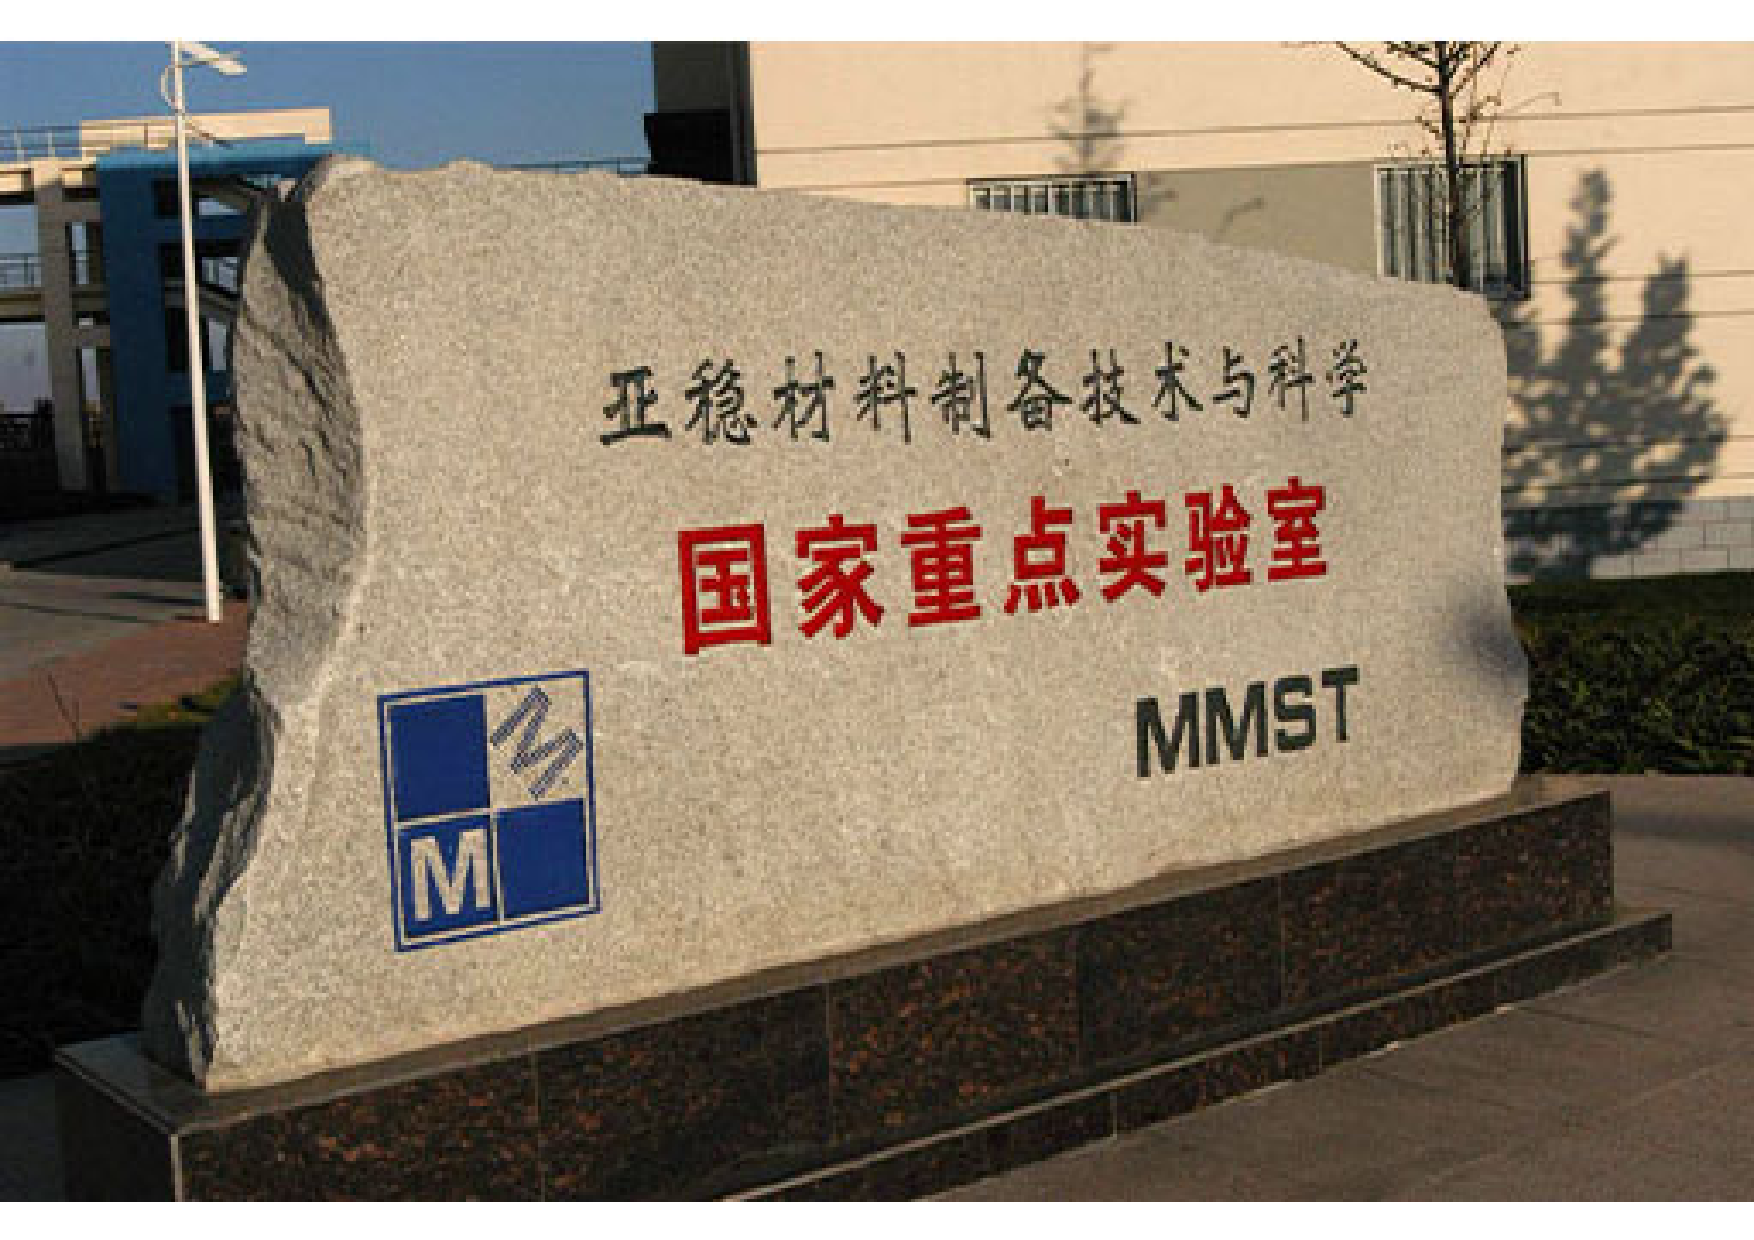
\includegraphics[width=0.4\textwidth]{亚稳材料制备技术与科学国家重点实验室.pdf}}
				\subcaptionbox{精品钢铁生产工艺装备智能化省部共建协同创新中心\label{fig_finesteel}}[0.49\textwidth]{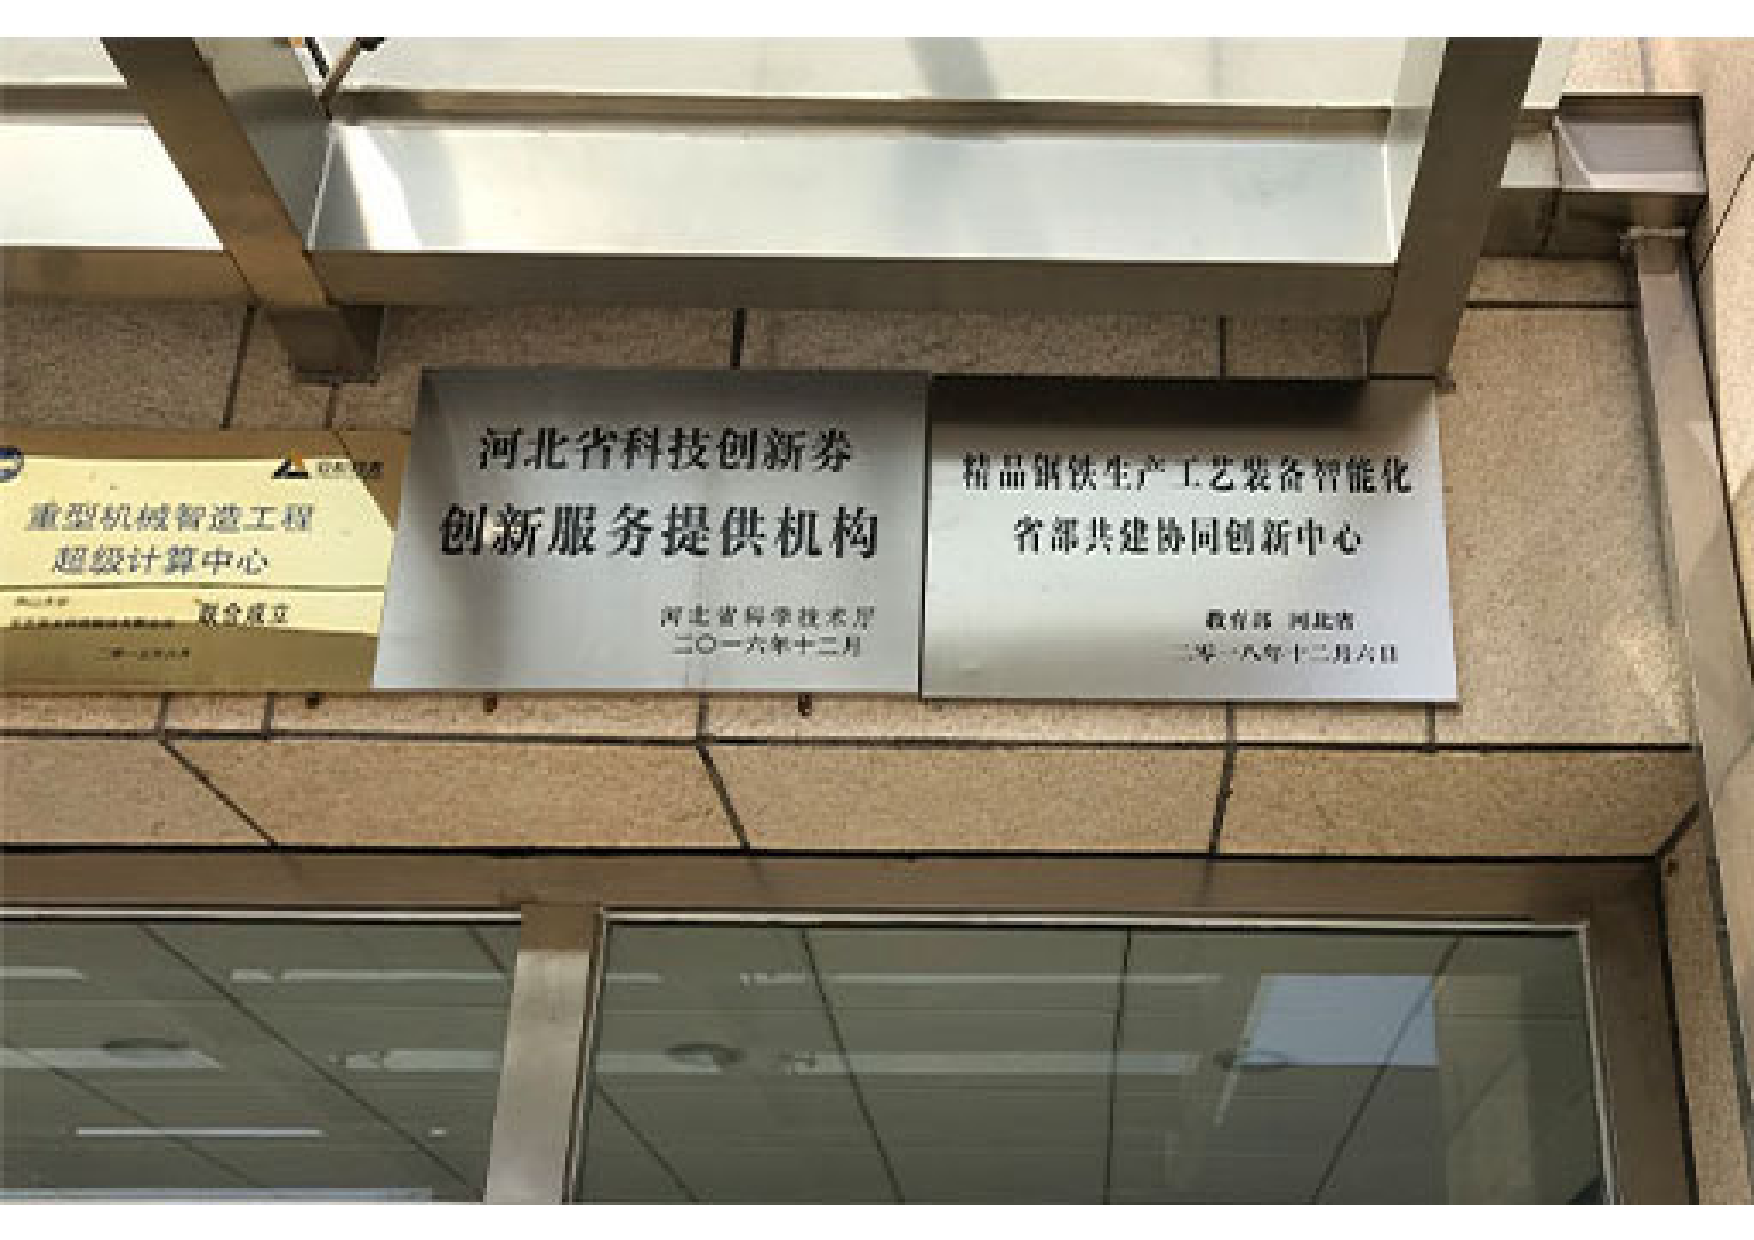
\includegraphics[width=0.4\textwidth]{精品钢铁生产工艺装备智能化省部共建协同创新中心.pdf}}
				\subcaptionbox{国家创新人才培养示范基地\label{fig_innovativetalents}}[0.49\textwidth]{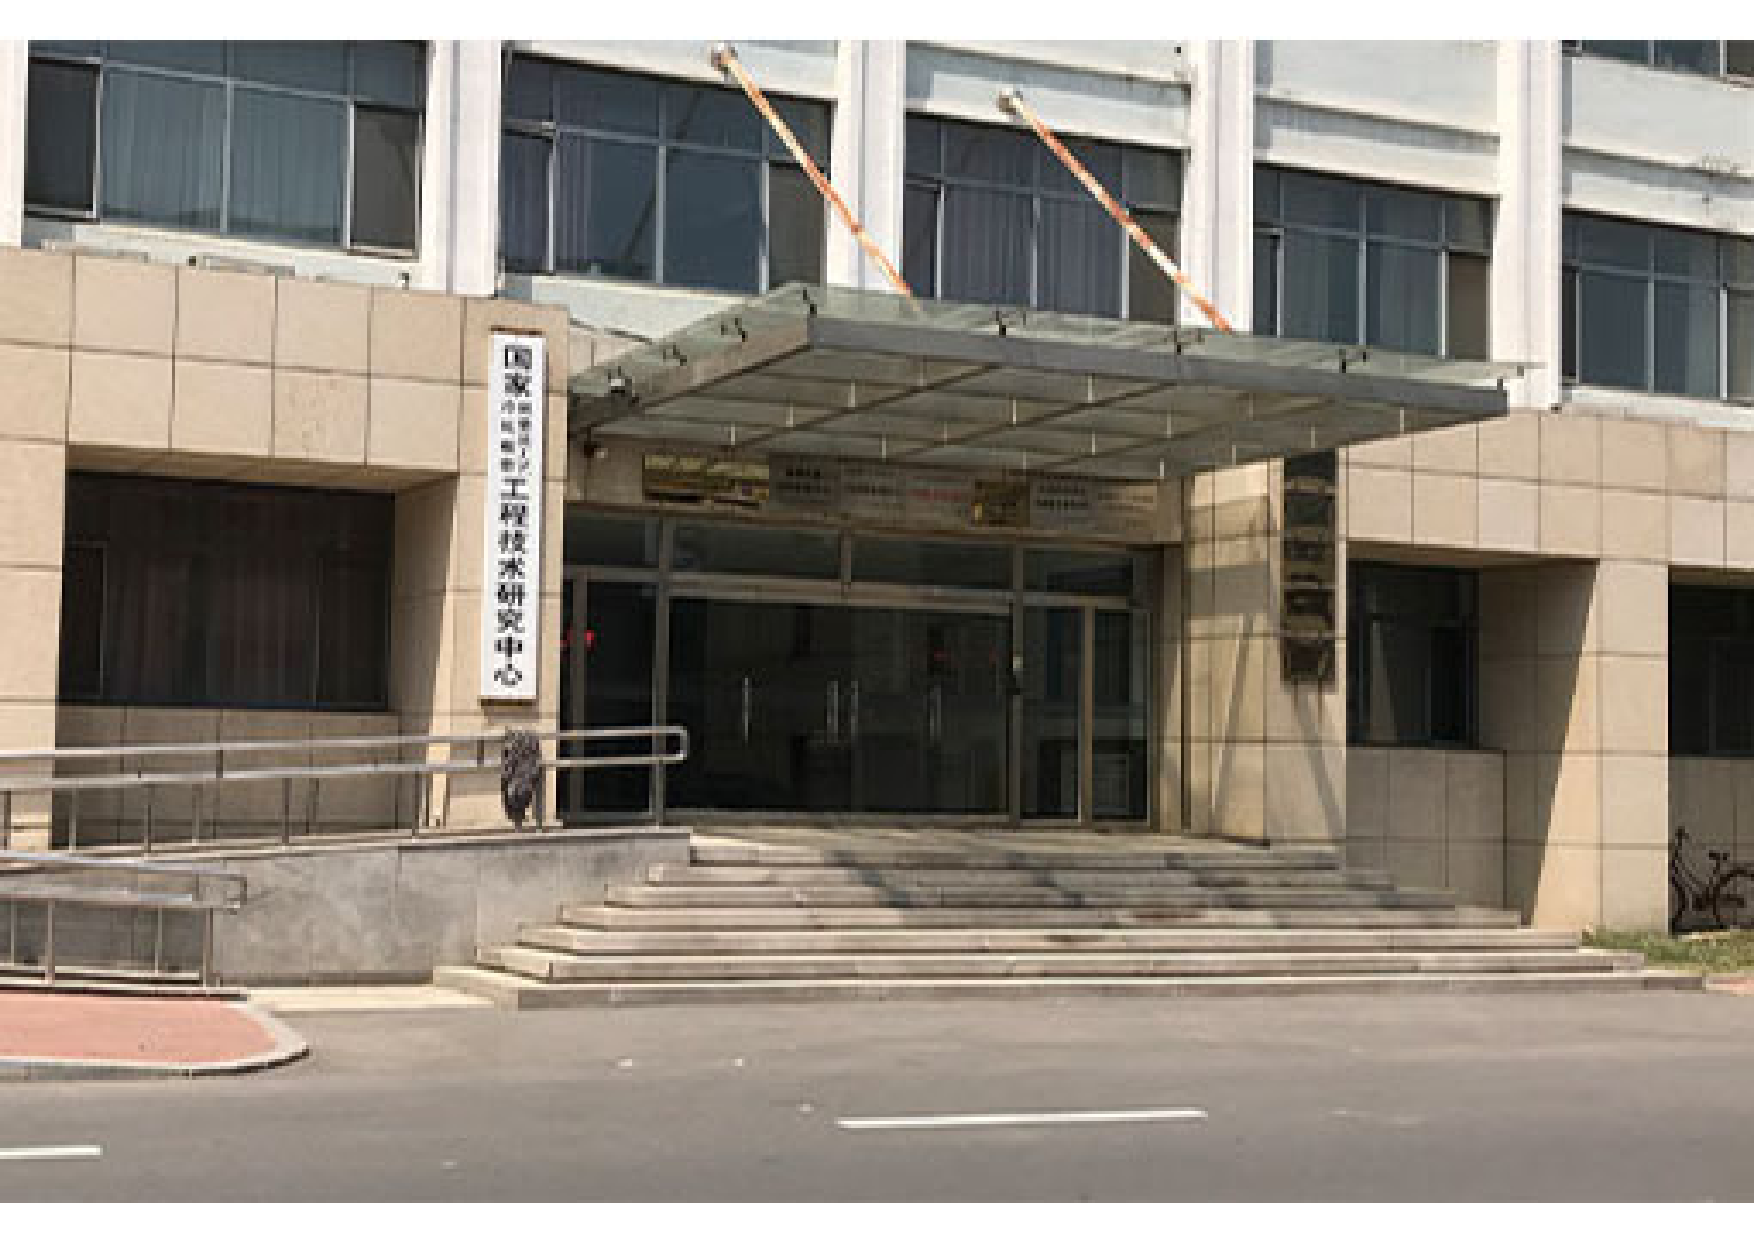
\includegraphics[width=0.4\textwidth]{国家创新人才培养示范基地.pdf}}
				\subcaptionbox{国家冷轧板带装备及工艺工程技术研究中心\label{fig_coldrolledstrip}}[0.49\textwidth]{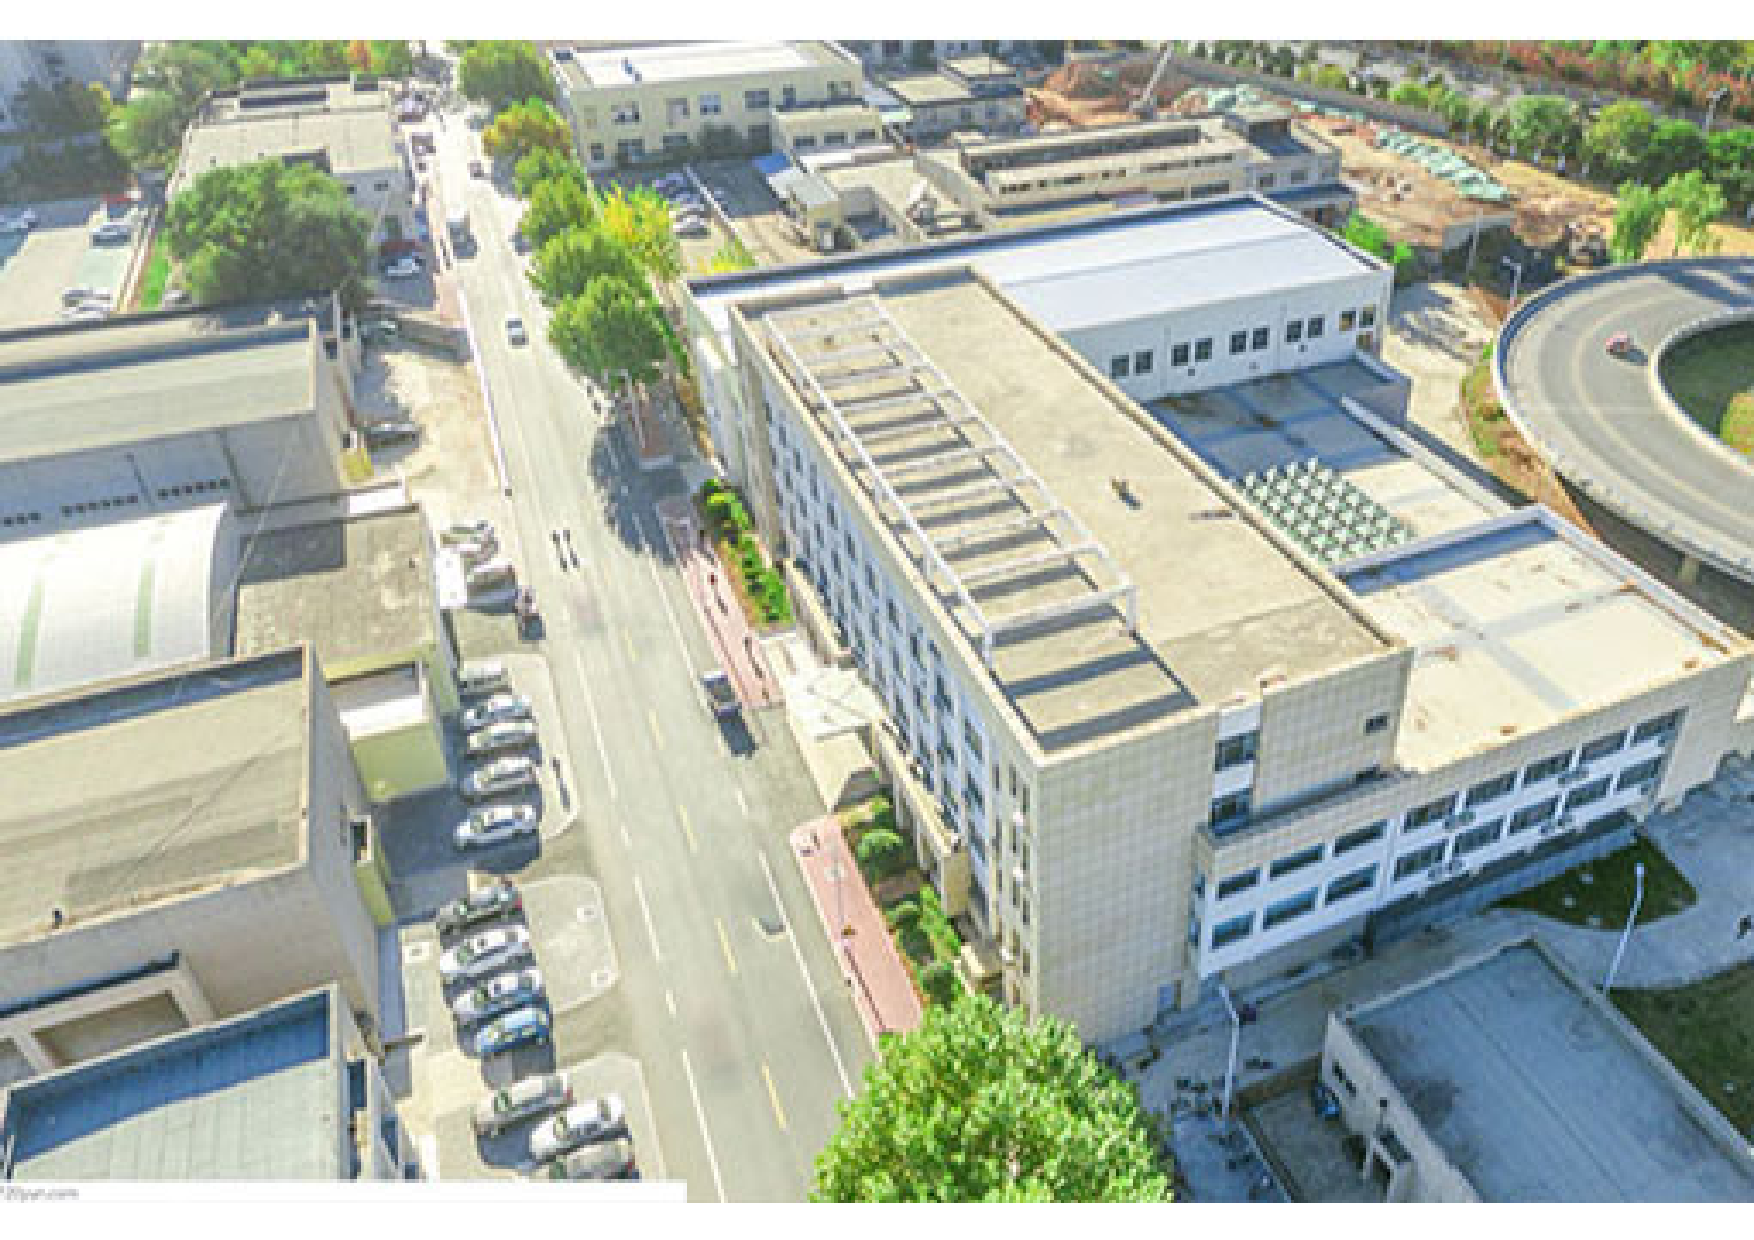
\includegraphics[width=0.4\textwidth]{国家冷轧板带装备及工艺工程技术研究中心.pdf}}
				\caption{燕山大学国家基地}
				\label{fig_ysunationalbase}
			\end{figure}
			
			\begin{figure}[!ht]
				\centering
				\bisubcaptionbox{亚稳材料制备技术与科学国家重点实验室\label{fig_bi_mmst}}{State Key Laboratory of Metastable Materials Science and Technology}[0.49\textwidth]{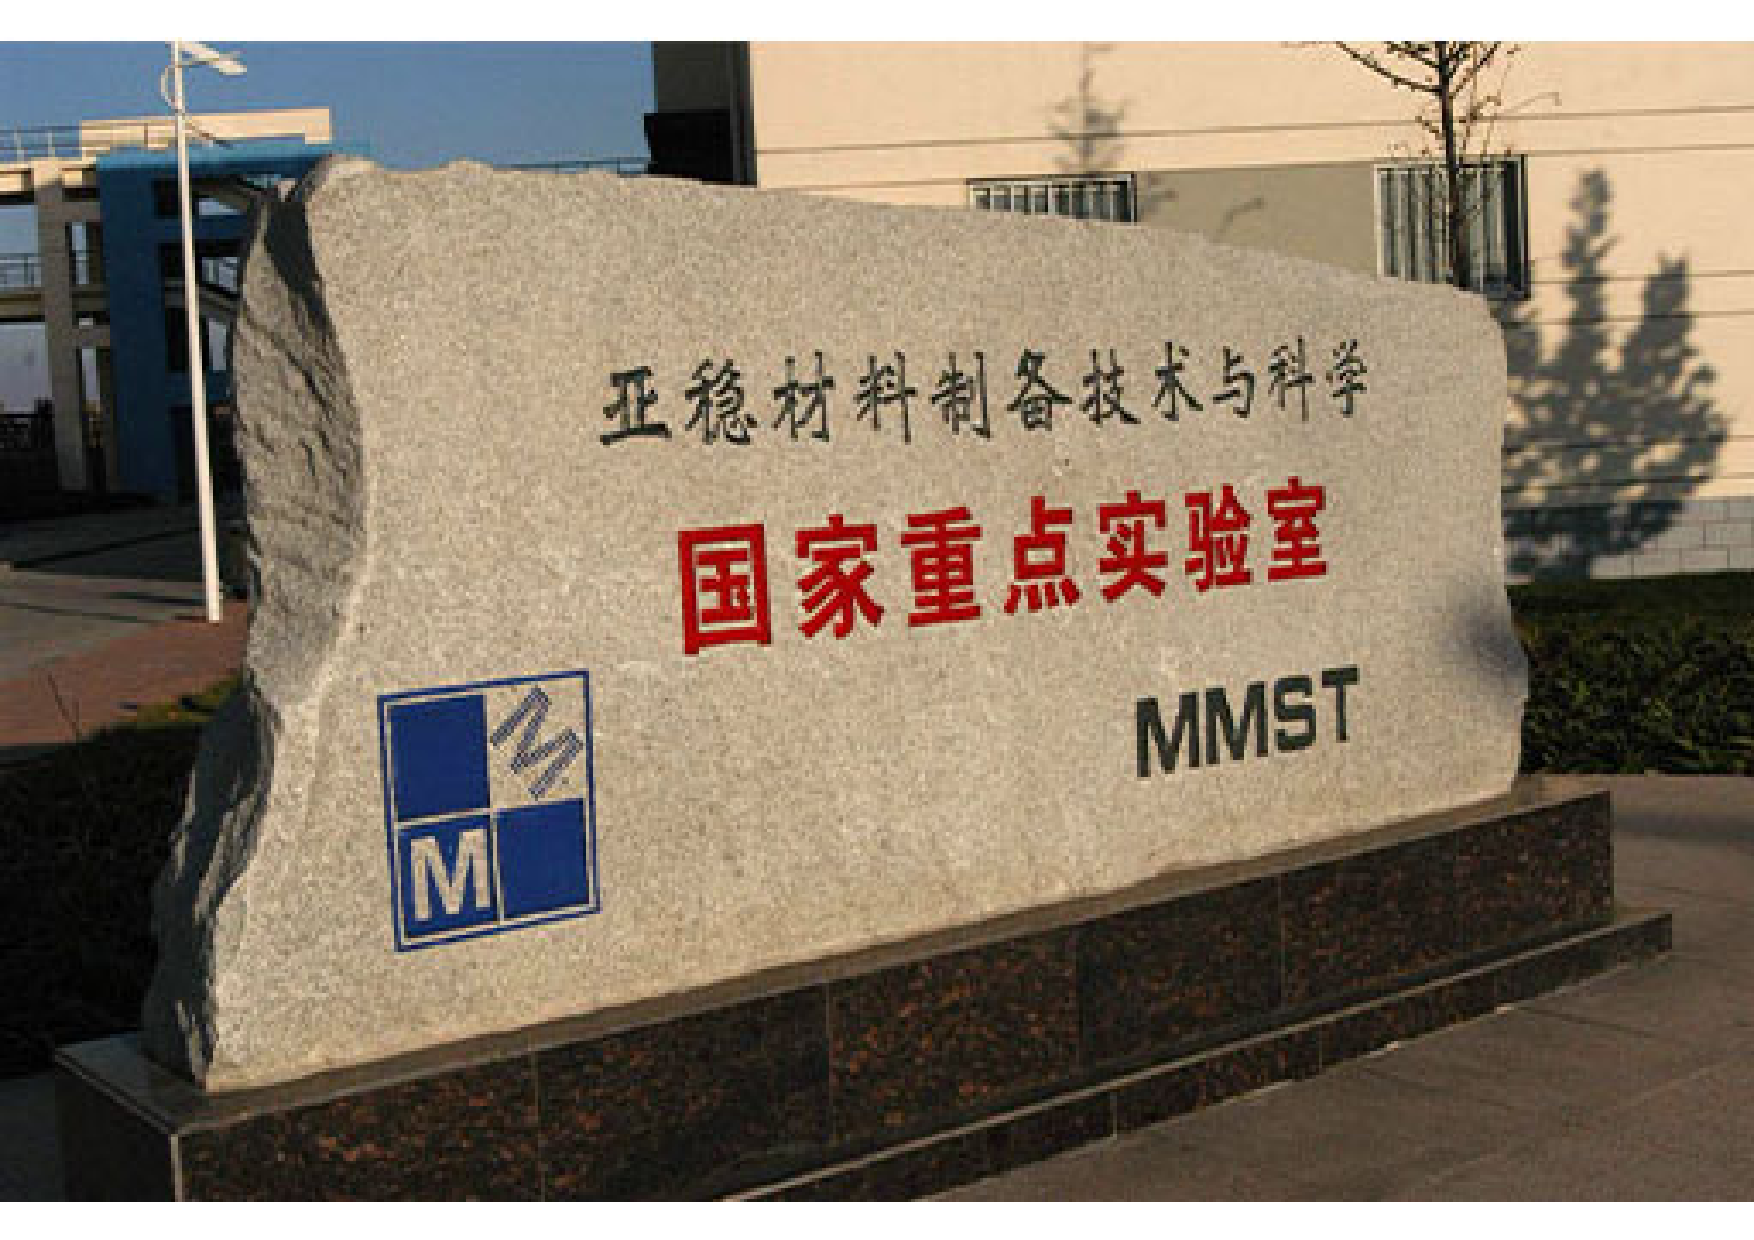
\includegraphics[scale=0.25]{亚稳材料制备技术与科学国家重点实验室.pdf}}
				\bisubcaptionbox{精品钢铁生产工艺装备智能化省部共建协同创新中心\label{fig_bi_finesteel}}{High-quality iron and steel production process equipment intelligence, the Ministry of Chemical Cooperation and Innovation Center}[0.49\textwidth]{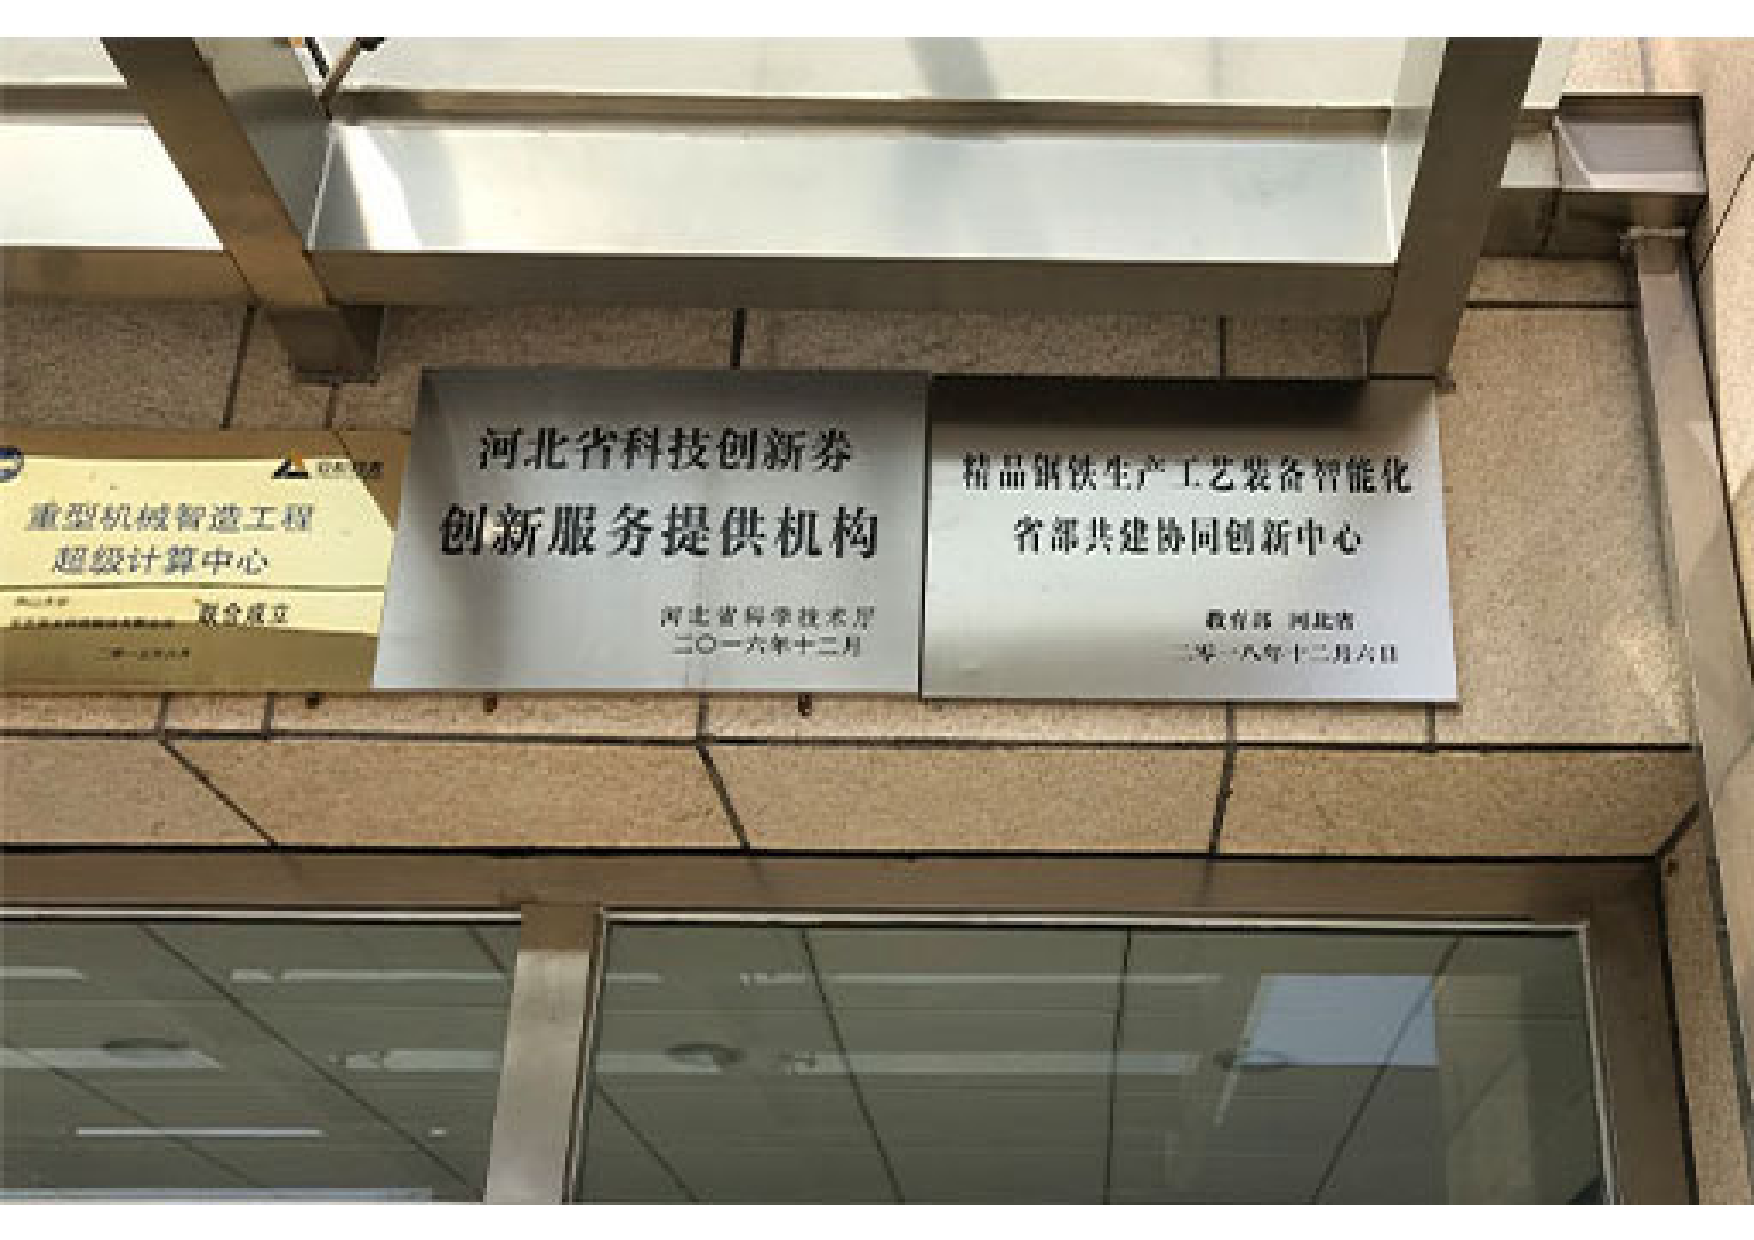
\includegraphics[scale=0.25]{精品钢铁生产工艺装备智能化省部共建协同创新中心.pdf}}
				\bisubcaptionbox{国家创新人才培养示范基地\label{fig_bi_innovativetalents}}{National Demonstration Base for training innovative talents}[0.49\textwidth]{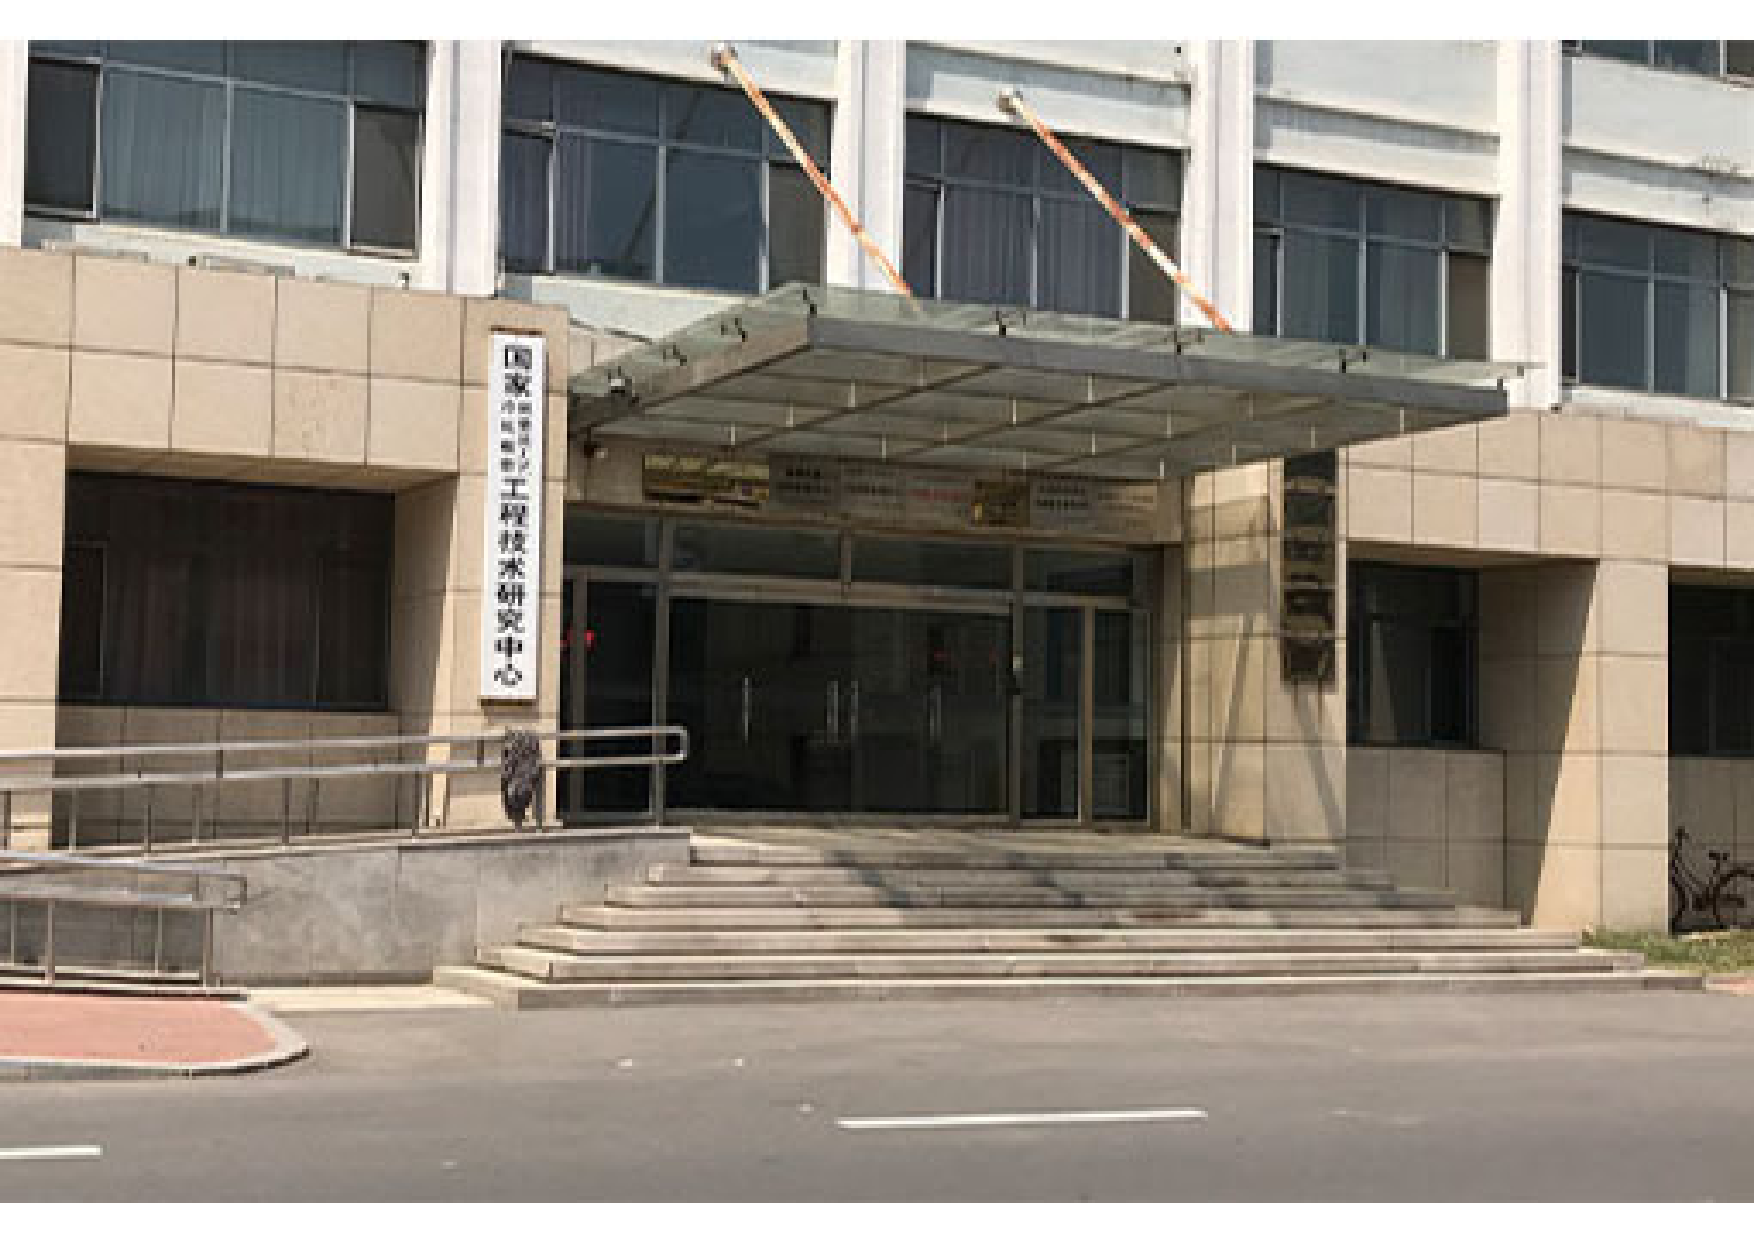
\includegraphics[scale=0.25]{国家创新人才培养示范基地.pdf}}
				\bisubcaptionbox{国家冷轧板带装备及工艺工程技术研究中心\label{fig_bi_coldrolledstrip}}{National Research Center for cold-rolled strip equipment and technology}[0.49\textwidth]{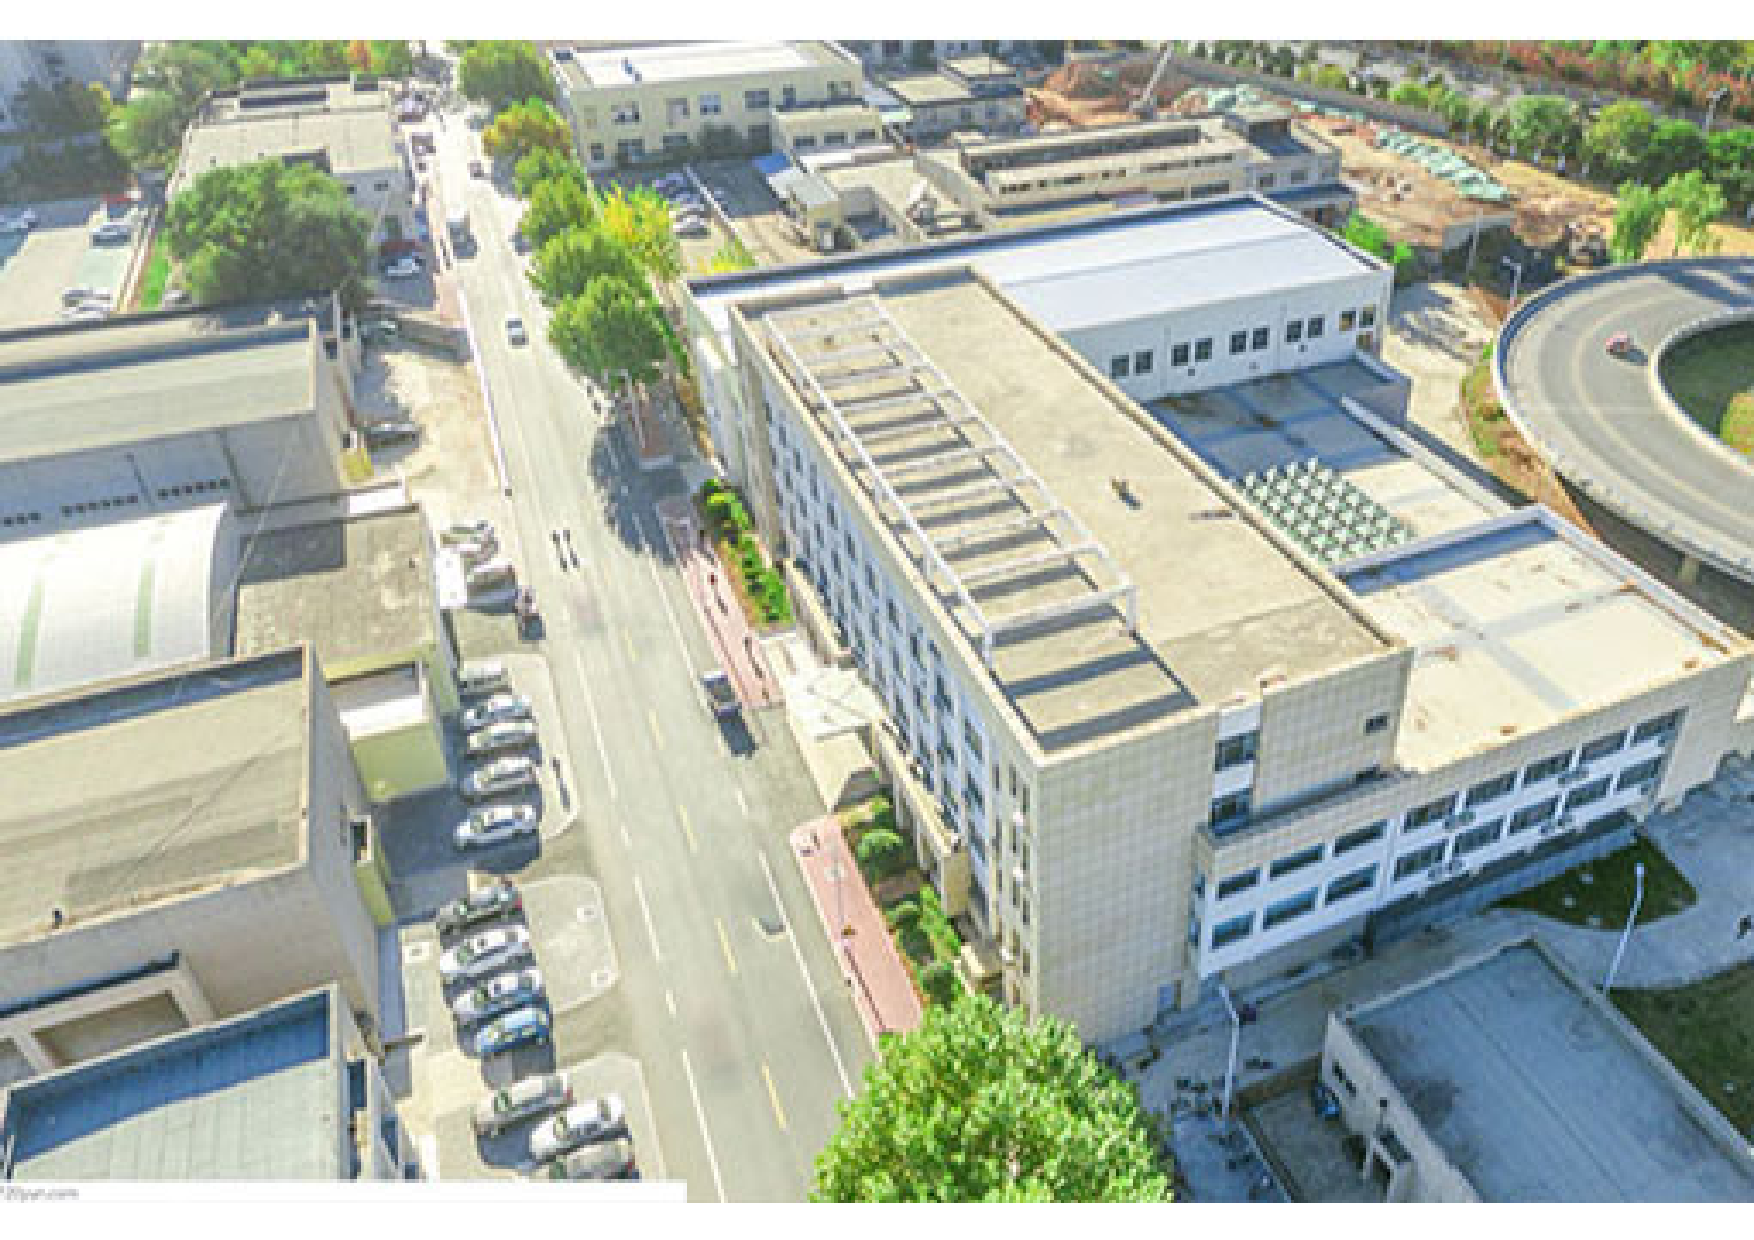
\includegraphics[scale=0.25]{国家冷轧板带装备及工艺工程技术研究中心.pdf}}
				\bicaption{燕山大学国家基地}{The national base of Yanshan University}
				\label{fig_bi_ysunationalbase}
			\end{figure}
		%-------------------插入多张图片示例结束-------------------


		下面是插入行内公式的示例。

		勾股定理$a^2+b^2=c^2$也被称为商高定理。

		下面是插入行间公式的示例。

		公式\eqref{eq:a^2+b^2}可以根据公式\eqref{eq:a}和\eqref{eq:b}得到。

		\begin{align}
			\theta&=\omega t\notag\\
			a&=\cos\theta \label{eq:a}\\
			b&=\sin\theta \label{eq:b}\\
			a^2+b^2&=1
			\label{eq:a^2+b^2}
		\end{align}

		式\eqref{eq2:a^2+b^2}可由式\eqref{eq2:identity_a_b}得出。
		\begin{subequations}
			\label{eq2:identity_a_b}
			\begin{align}
				\theta&=\omega t\notag\\
				a&=\cos\theta \label{eq2:a}\\
				b&=\sin\theta \label{eq2:b}\\
				a^2+b^2&=1
				\label{eq2:a^2+b^2}
			\end{align}
		\end{subequations}

		表\ref{tab_para1}~为插入表格示例。

		%--------------插表示例开始--------------
		\begin{table}[!ht]
			\caption{System Parameters}
			\label{tab_para1}
			\centering
			\begin{tabular}{CLR}
				\toprule
				Parameter & Description & Value \\
				\midrule
				$L$ & filter inductance & $2\mathrm{mH}$ \\
				$C$ & filter capacitance & $100\mu\mathrm{F}$ \\
				$R$ & load resistance & $10\Omega$ \\
				\bottomrule
			\end{tabular}
		\end{table}
		%--------------插表示例结束--------------
		\begin{table}[!ht]
			\bicaption{博士中文表题}{System Parameters}
			\label{tab_para2}
			\centering
			\begin{tabular}{CLR}
				\toprule
				Parameter & Description & Value \\
				\midrule
				$L$ & filter inductance & $2\mathrm{mH}$ \\
				$C$ & filter capacitance & $100\mu\mathrm{F}$ \\
				$R$ & load resistance & $10\Omega$ \\
				\bottomrule
			\end{tabular}
		\end{table}

	\chapter{无人铰接车微分平坦全局轨迹规划方法}

		在传统的全局规划问题中,目标是找到从起点到终点的最优路径,最优的指标一般是路径最短。例如A*算法和Dijstra算法可以在栅格地图中搜索出路径代价最小的路径,RRT*系列算法在概率完备下得到路径也是距离最短的。然而,这些全局规划算法并不会考虑车身的朝向和曲率等信息。它们仅仅针对全向或者差速机器人会非常有效,面对具有强非完整性的机器人来说就显得吃力了。考虑以下场景地图的算法搜索特例:  
		\begin{figure}[!ht]
			\centering
			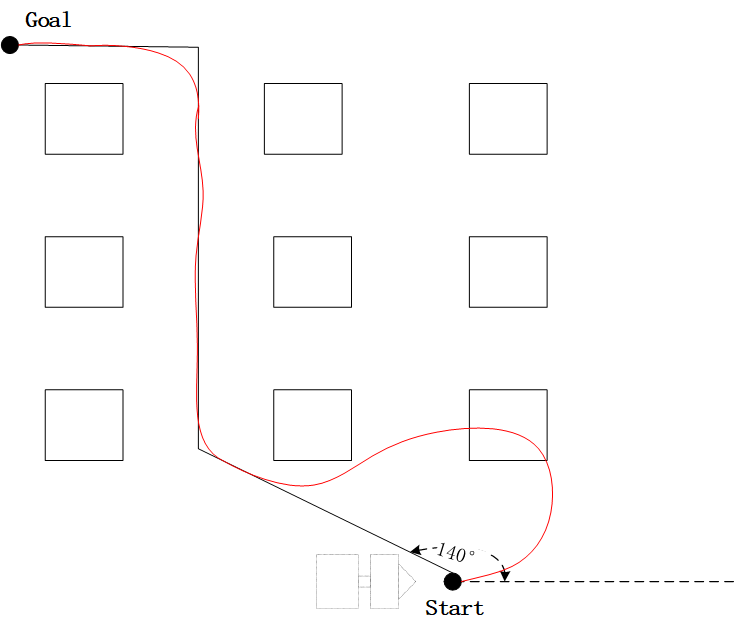
\includegraphics[width=0.8\textwidth]{路径规划算法特例.png}
			\caption{路径规划算法特例}
			\label{fig:路径规划算法特例}
		\end{figure}
		上图中时模拟一个路径规划算法的特殊例子,需要规划起点Start到终点Goal的路径。一般的算法可能规划出如图的路径,可以看到路径的起点切向和机器人的朝向相差140度。对于差速机器人跟踪这条路径的话,他会先原地转向然后继续跟踪其他点。对于全向机器人它直接可以顺着路径走,不必掉头。但是对于类车转向和铰接转向底盘,这两种底盘在转向时不仅有严格的非完整性,同时转向半径非常大。这会直接导致在开始的一段路径跟踪时会走出如图红色的路径,严重不贴合全局路径。这会带来出乎意料的后果,例如撞向障碍物或走出地图边缘。
		%然而,在具体的工作场景中,例如码头搬运任务,铰接车通常需要采用一种面向任务的路径规划方法。例如,车辆需要先到达A点进行货物装载,然后再前往B点进行卸货。/
		本章将基于优化理论和Minco样条,提出一种适用于铰接车辆的全局路径优化方法,可以在整段路径上保证严格的转弯半径约束并保证安全躲避碰撞。
		

	\section{铰接模型微分平坦性}
		\subsection{铰接车运动学模型的分析}
		铰接车总体上一共由前桥和后桥组成,中间通过液压或者舵机驱动铰接角完成转向。本文介绍的铰接车运动学模型如下:  
		%图片  
		\begin{figure}[!ht]
			\centering
			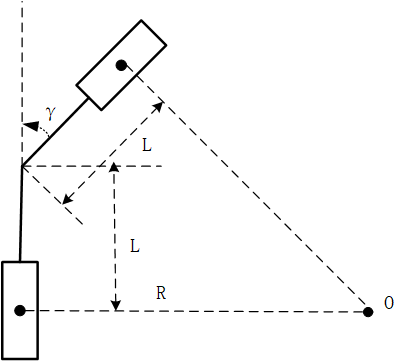
\includegraphics[width=0.8\textwidth]{铰接车简易模型.png}
			\caption{铰接车简易模型}
			\label{fig:铰接车简易模型}
		\end{figure}
		如上图所示,我们假设前轴中点作为参考点,前轴的航向角为theta1,后轴航向角为theta2。其中o点为瞬时转向圆心,pf为前轴中点pr为后轴中点,lf是前轴长度,lr是后轴长度,gamma是铰接角。为了推出铰接车的运动学模型,我们做出以下两个假设。(1)铰接车辆始终保持低速运动,忽略动力学特性。(2)假设车辆不发生侧滑。
		首先由于车辆不会发生打滑,所以车辆运动时前后车轮完全满足车辆的滚动约束,即速度方向和车辆的朝向保持一致。得到以下方程:
		
		\begin{equation}
			\begin{aligned}
				&\dot{x}_1=vcos\theta _1\\
				&\dot{y}_1=vsin\theta _1\\
				&\dot{x}_1sin\theta _1-\dot{y}_1cos\theta _1=0\\
				&\dot{x}_2sin\theta _2-\dot{y}_2cos\theta _2=0
			\end{aligned}
		\end{equation}
		由于前桥和后桥通过铰接角刚性连接,我们可以推导出前桥参考点和后桥参考点的坐标变换公式如下:
		\begin{equation}
			\begin{aligned}
				&x_1=x_2+l_2cos\theta _2+l_1cos\theta _1\\
				&y_1=y_2+l_2sin\theta _2+l_1sin\theta _1\\
				&\theta _2=\theta _1-\gamma 
			\end{aligned}
		\end{equation}
		以前桥为参考点,定义$(x,y,theta,gamma)$为铰接车的位姿,他们分别代表着$x_f,y_f,\theta,\gamma$。在我们的研究中铰接车的前桥和后桥相等,即$lf=lr=L=1.3m$。联合上式我们可以得到铰接车的运动学方程为:
		\begin{equation}
			\begin{aligned}
				\frac{d}{dt}\left[ \begin{array}{c}
					x_f\\
					y_f\\
					\theta\\
					\gamma\\
				\end{array} \right] =\left[ \begin{array}{c}
					vcos\theta\\
					vsin\theta\\
					vtan( \gamma /2 ) /L+\omega /( cos\gamma +1 )\\
					\omega\\
				\end{array} \right] 
			\end{aligned}
		\end{equation}
		其中$v,w$是输入量,分别代表这前轴速度和铰接角速度。
		\subsection{铰接车模型的平坦输出}
		在实际场景中情况是非常复杂的,全局的轨迹规划中我们不需要用精确的运动学模型。在这里我们忽略动态转向,只保留静态转向模型。假设 为系统输入,静态转向模型为:
		\begin{equation}
			\begin{aligned}
				\dot{\theta}=v\frac{tan( \gamma /2 )}{L}
			\end{aligned}
		\end{equation}
		对于一个非线性系统的动态方程具有如下一般的表达形式:
		\begin{equation}
			\begin{aligned}
				\dot{x}&=f( x,u ) ,x\in R^n,u\in R^m\\
			\end{aligned}
		\end{equation}
		其中$x$是状态变量,$f(x,u)$是系统的非线性函数。对于一个非线性系统,如果能找一组输出变量,使得所有的状态变量输出变量都可以用这组输出变量及其多阶导数所表示,则称这个系统为微分平坦系统。
		对于微分平坦的运动学模型,其平坦输出一般具有实际的物理意义往往会给问题带来很好的可表征性。对于铰接车的运动模型,我们选择$x,y$作为平坦输出,这在轨迹规划中可以带来很好的性质。
		下面我们给出装载机的微分平坦系统:
		\begin{equation}
			\begin{aligned}
				v&=\eta \sqrt{\dot{x}^2+\dot{y}^2},\\
				\theta &=arctan2( \eta \dot{y},\eta \dot{x} ) ,\\
				\gamma &=2arctan( \eta ( \dot{x}\ddot{y}-\dot{y}\ddot{x} ) L/( \dot{x}^2+\dot{y}^2 ) ^{\frac{3}{2}} ) ,\\
				k&=( \dot{x}\ddot{y}-\dot{y}\ddot{x} ) /( \dot{x}^2+\dot{y}^2 ) ^{\frac{3}{2}}.\\
			\end{aligned}
		\end{equation}
	其中$x,y$是系统的平坦输出变量,$(v,theta,gamma,k)$是我们选取的状态变量。k为轨迹的曲率,值得指出的是曲率其实也是铰接角的函数,但是这里只在路径层面说明。$n\in{1,-1}$是车辆运动的方向,分别代表前进和后退两种情况。
	\section{参数化轨迹表达形式}
	在自动驾驶中参数化曲线的方法有很多,例如五次多项式、贝塞尔曲线、B样条、螺旋线、Dubin曲线和RS曲线。MINCO曲线作为是一种基于五次多项式的曲线类型,它在处理微分平坦系统上有着天然的优势【文献】。我们这一小节将介绍minco曲线的原理,并且运用它处理我们的铰接模型运动规划问题。
		\subsection{MINCO曲线轨迹原理}
		铰接车在静态转向时表现出微分平坦性,这意味着其运动学微分约束可以通过一组平坦变量及其多阶导数来表示。在多项式规划中一个典型的BVP问题可以表示为:
		\begin{equation}
			\begin{aligned}
				min\int_0^T{v}(t) ^TWv(t) dt\\
				s.t. \ \ \ z^s(t) =v(t) ,\forall t\in \left[ 0,T \right] ,\\
				z^{\left[ s-1 \right]}( t_0 ) =\bar{z}_o,z^{\left[ s-1 \right]}( t_M ) =\bar{z}_f.
			\end{aligned}
		\end{equation}
		其中$z(t)$是参数曲线,$v(t)$是$z(t)$关于时间的$s$阶导数,$z_0$和$z_f$分别是起点和终点。对于以上最小控制输入问题,若系统是微分平坦的,且最小控制量是平坦变量的$s$阶次导数,则BVP问题的最优解是一个$2s-1$次多项式【文献】。特殊的,当$s=3$时这是一个minimumJerk(最小化加加速度代价)问题,他的最优解是一个五次多项式。 
		综上,轨迹曲线$z(t)$可以被表示为关于时间$t$多项式函数$\beta(t)$:
		\begin{equation}
			\begin{aligned}
				z=\beta (t) =\lambda ^T(t) c=c_0+c_1t+c_2t^2+c_3t^3+c_4t^4+c_5t^5\\
				=\left[ 1\,\,t\,\,\,\,t^2\,\,t^3\,\,t^4\,\,t^5 \right] \cdot \left[ c_0\,\,c_1\,\,c_2\,\,c_3\,\,c_4\,\,c_5 \right] ^T
			\end{aligned}
		\end{equation}
		其中$c$是多项式的系数向量。这个多项式由起点和终点的各阶状态量解出。假设轨迹的时间段是$T$,写成矩阵形式:
		\begin{equation}
			\begin{aligned}
				\left[ \begin{array}{c}
				x_s\\
				v_s\\
				a_s\\
				x_e\\
				v_e\\
				a_e\\
				\end{array} \right] =\left[ \begin{matrix}
				1&		0&		0&		0&		0&		0\\
				0&		1&		0&		0&		0&		0\\
				0&		0&		2&		0&		0&		0\\
				1&		T&		T^2&		T^3&		T^4&		T^4\\
				0&		1&		2T&		3T^2&		4T^3&		5T^4\\
				0&		0&		2&		6T&		12T^2&		20T^3\\
				\end{matrix} \right] \left[ \begin{array}{c}
				c_0\\
				c_1\\
				c_2\\
				c_3\\
				c_4\\
				\end{array} \right] ==>d=A_F(t) c
			\end{aligned}
		\end{equation}
		在上式中,$x_s,v_s,a_s$分别是轨迹起点的位置、速度和加速度,$x_e,v_e,a_e$对应为终点的状态。在实际的规划问题中为了保证轨迹的灵活性,轨迹规划被表述为多个BVP的总和,即BIVP问题:
		\begin{equation}
			\begin{aligned}
				\min_{z(t)}\int_{t_0}^{t_M}&v^T(t)\mathbf{W}v(t)dt\\
				\text{s.t}.z^{( s )}(t) &=v(t) \quad \forall t\in \left[ t_0,t_M \right]\\
				z^{\left[ s-1 \right]}( t_0 ) &=\bar{z}_o,z^{\left[ s-1 \right]}( t_M ) =\bar{z}_f\\
				z^{\left[ d_i-1 \right]}( t_i ) &=\bar{z}_i,1\leq i<M\\
				t_{i-1}&<t_i,1\leq i\leq M.\\
			\end{aligned}
		\end{equation}
		MINCO给出了这个BIVP问题的最优解形式,其最优性条件指出:对与最小化$s$阶导数的BIVP问题,他的最优解的单段轨迹一定是一个$2s-1$次多项式,且这个解具有$s+1$阶导数的连续性【文献】。这意味着我们在处理minimumJerk(s = 3)的轨迹时,这个轨迹具有snap阶(s = 4)阶的连续性,则BIVP问题的闭式解完全可以由起点状态、终点状态和中间位置所得到,如图..。
		\begin{figure}[!ht]
			\centering
			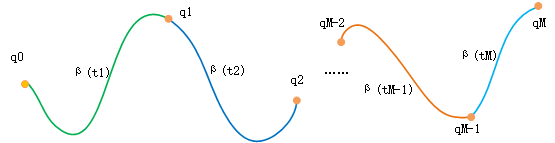
\includegraphics[width=0.8\textwidth]{minco.png}
			\caption{minco}
			\label{fig:minco}
		\end{figure}
	
		\subsection{轨迹参数化过程}
		假设我们共有$M+1$个航点$q_0~q_M$,其中起点$q_0=[x_s,y_s,v_{sx},v_{sy},a_{sx},a_{sy}]$和终点$q_M=x_e=[x_e,y_e,v_{ex},v_{ey},a_{ex},a_{ey}]$完全已知,需要求出M段多项式轨迹的表达式。  
		   
			A、起点和终点约束    
			  
			我们假设s=3,一个规划问题的起点和终点是已知的,起点和终点可以得到一共可以得到2s=6个约束方程,起点的约束方程为:
			\begin{equation}
				\begin{aligned}
				\left[ \begin{matrix}
					p_{0x}&		p_{0y}\\
					v_{0x}&		v_{0y}\\
					a_{0x}&		a_{0_y}\\
				\end{matrix} \right] =\left[ \begin{matrix}
					1&		0&		0&		0&		0&		0\\
					0&		1&		0&		0&		0&		0\\
					0&		0&		2&		0&		0&		0\\
				\end{matrix} \right] \left[ \begin{matrix}
					c_{0x}^{0}&		c_{0y}^{0}\\
					c_{1x}^{0}&		c_{1y}^{0}\\
					c_{2x}^{0}&		c_{2y}^{0}\\
					c_{3x}^{0}&		c_{3y}^{0}\\
					c_{4x}^{0}&		c_{4y}^{0}\\
					c_{5x}^{0}&		c_{5y}^{0}\\
				\end{matrix} \right] ==>b_0=F_0\cdot c_0
				\end{aligned}
			\end{equation}
			
			B、航点的连续性约束
			
			除了已知起点和终点之外,我们还必须保证BIVP问题中间航点的连续性。根据Minco的理论,minimumJerk问题(s=3)具有snap阶的连续性:
			\begin{equation}
				\begin{aligned}
					\left[ \begin{array}{c}
						\beta(t)\\
						\beta^{'}(t)\\
						\beta^{''}(t)\\
						\beta^{'''}(t)\\
						\beta^{''''}(t)\\
					\end{array} \right] &=\left[ \begin{array}{c}
						x(t)\\
						v(t)\\
						a(t)\\
						jerk(t)\\
						snap(t)\\
					\end{array} \right] =\left[ \begin{array}{c}
						\lambda_{t}^{T}\\
						\lambda_{t}^{( 1 ) T}\\
						\lambda_{t}^{( 2 ) T}\\
						\lambda_{t}^{( 3 ) T}\\
						\lambda_{t}^{( 4 ) T}\\
					\end{array} \right] \cdot \mathbf{c}=\left[ \begin{matrix}
						1&		t&		t^2&		t^3&		t^4&		t^5\\
						0&		1&		2t&		3t^2&		4t^3&		5t^4\\
						0&		0&		2&		6t&		12t^2&		20t^3\\
						0&		0&		0&		6&		24t&		60t^2\\
						0&		0&		0&		0&		24&		120t\\
					\end{matrix} \right] \cdot \mathbf{c}\\
					&\Longrightarrow G(t) \mathbf{c}=\mathbf{b}(t) 
				\end{aligned}
			\end{equation}
			因此第$i$段轨迹和第$i+1$段轨迹的连续性约束方程可以写为:
			\begin{equation}
				\begin{aligned}
					\left[ \begin{matrix}
						\beta ( T_i )&		0\\
						G( T_i )&		-G( 0 )\\
					\end{matrix} \right] \cdot \left[ \begin{array}{c}
						\mathbf{c}( i )\\
						\mathbf{c}( i+1 )\\
					\end{array} \right] =\left[ \begin{array}{c}
						\mathbf{b}( T_i )\\
						0\\
					\end{array} \right] \\
					\Longrightarrow \left[ E_i,F_i \right] \cdot \left[ \begin{array}{c}
						\mathbf{c}( i )\\
						\mathbf{c}( i+1 )\\
					\end{array} \right] =\left[ \begin{array}{c}
						\mathbf{b}( i )\\
						0\\
					\end{array} \right] 
				\end{aligned}
			\end{equation}
			综合起点、终点和航点的约束我们可以得到$2Ms$个约束方程,系数矩阵我们表示为M,由$M$和$b$可以唯一确定一组多项式系数$c$,即轨迹的参数形式。
			\begin{equation}
				\begin{aligned}
					M_{2Ms\cdot2Ms}\mathbf{c}=b\Longrightarrow ( \begin{matrix}
						\mathbf{F}_0&		0&		0&		\cdots&		0\\
						\mathbf{E}_1&		\mathbf{F}_1&		0&		\cdots&		0\\
						0&		\mathbf{E}_2&		\mathbf{F}_2&		\cdots&		0\\
						\vdots&		\vdots&		\vdots&		\ddots&		\vdots\\
						0&		0&		0&		\cdots&		\mathbf{F}_{M-1}\\
						0&		0&		0&		\cdots&		\mathbf{E}_M\\
					\end{matrix} ) \cdot \left[ \begin{array}{c}
						\mathbf{c}_1\\
						\mathbf{c}_2\\
						\mathbf{c}_3\\
						\vdots\\
						\mathbf{c}_{M-1}\\
						\mathbf{c}_M\\
					\end{array} \right] =\left[ \begin{array}{c}
						b_0\\
						b( 1 )\\
						0\\
						\vdots\\
						0\\
						b_M\\
					\end{array} \right] 
				\end{aligned}
			\end{equation}
			值得一提的是,在$M$矩阵中$T_i$是第$i$段多项式的总时间,它可以提前由一些其他的算法来给出,这样M就是完全已知的矩阵了。由于我们做的是路径规划,所以我们把$T_i$都归一化处理作为常数。
			
		\subsection{轨迹平滑与优化}
		常见的路径规划算法得到的路径是有拐角的,对于具有转向半径约束的车辆来说并不能完全的跟踪。因此在进行轨迹规划时必须考虑最大曲率的约束条件:
		\begin{equation}
			\begin{aligned}
				k_{max}=\frac{1}{R_{max}}=\frac{tan( \gamma _{max}/2 )}{L}
			\end{aligned}
		\end{equation}
	
	\section{轨迹的避障约束分析}
	在上一节中我们已经对铰接车的轨迹进行了参数化,这样就自然的处理了微分方程带来的约束问题,保证了轨迹的平滑性。无人车辆在非结构或半结构的场景中还需要面临安全性带来的种种挑战,包括避开其他工程机械车辆和环境中的种种障碍物。无人车的避障和地图的表示形式是分不开的,常见的地图表示方法有占据栅格地图、点云地图、距离场、特征地图、拓扑地图、场图以及语义地图。规划算法中的避障部分一般根据地图的表示差异而有所不同。对于栅格地图而言,由于其均匀的栅格大小和快速的索引方式,使得它在几乎所有的避障算法中首当其冲,例如ROS(robot Operte sys。。)框架中就实现了基于栅格地图搜索的A*算法和Dijstra算法。点云地图是对空间中障碍物的直接表示,常见的激光slam算法建立的地图一般都是这种类型,基于此种地图的规划器一般需要结合KDTree(最近邻)搜索离当前位置最近的障碍物并避开。其次是特征地图,特征地图并不对整个地图空间进行离散,而是在地图上仅仅保留稀疏的特征。这些地图类型在不同的场景下有着不同的优势,针对某种类型的地图往往需要选择行之有效的规划器,减小规划的空间和时间复杂度。考虑到施工现场的结构不确定,往往地面上会有许多的杂物,为了充分表征这些障碍物从而达到安全避障行驶的目的,我们选择使用2维空间下的占据栅格地图作为规划的地图类型。
		\subsection{凸多边形约束的数学表达}
		对于凸包地图区间一般有两种表示方法,一种是把障碍物的轮廓用一个凸多边形近似模拟。另一种是则相反,将地图中安全的区域用凸多边形近似。为了接收原始的点云地图,提高通用性,我们选择的方法是后者,将地图安全区域用凸多边形来近似。
		\begin{figure}[!ht]
			\centering
			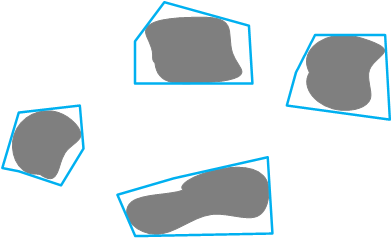
\includegraphics[width=0.8\textwidth]{凸包1.png}
			\caption{凸包1}
			\label{fig:凸包1}
		\end{figure}
		\begin{figure}[!ht]
			\centering
			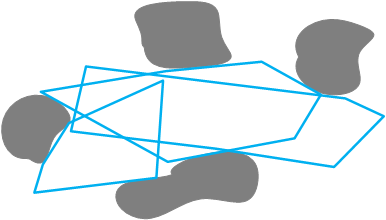
\includegraphics[width=0.8\textwidth]{凸包2.png}
			\caption{凸包2}
			\label{fig:凸包2}
		\end{figure}
		凸多边形的表示方法有很多种类型,例如矩形和不规则凸多边形。在广义上,球体和椭球体也属于凸体。我们选择的空间表示体是不规则凸多边形。凸多边形的区域由一组半空间交集组成,在空间内的点满足以下不等式约束:
		\begin{equation}
			\begin{aligned}
				H_z&=\{p\mid Ap<b\},\\
				A&=\left[ a_0,a_1 \right] _{n_z-1\times 2},b=\left[ b_0,...,b_z,...,b_{n_z-1} \right] ^T.
			\end{aligned}
		\end{equation}
		其中$a_i$是第$i$个半空间的法向量,$a_i$和$b_i$唯一去确定一个超平面约束。对于任意在多边形内的点应当满足【等式】带来的不等式约束。多边形的生成方法参看文献【】。
	
	\section{单阶段无约束轨迹规划}
	在3.2中我们介绍了MINCO曲线的参数化形式。由于我们在这一章介绍的全局的路劲规划,所以我们只关心路径层面信息包括曲率和避障。路径的最大曲率,这由装载机的最大转向角推导得到。避障我们在3.3节我们已近介绍。
		\subsection{优化问题的建立}
		针对于这个问题我们使用优化的方法解决,我们把曲率和安全约束离散化的施加在问题中,当离散化的点足够多时轨迹就是足够安全的。我们可以得到以下优化问题的表达形式:
		\begin{equation}
			\begin{aligned}
				&\min J( c )=0 \\
				s.t.\,\,&-k_{max}\le k_{ij}\le k_{max} \\
				&A_ip_{ij}<b_i,\ \ i\in \left[ 1,N \right] ,j\in \left[ 1,m_i \right] 
			\end{aligned}
		\end{equation}
		其中$c$轨迹多项式是系数矩阵,$K_{max}$是最大曲率,$N$是轨迹的段数,$m_i$是第$i$段轨迹的离散点数,$p_{ij}$是第$i$点轨迹的第$j$个点。
		\subsection{曲率约束和避障约束的消除}
		忽略动态转向带来的曲率影响,铰接式车辆的最大曲率由静态转向模型确定。本次设计中我们的最大转向角度为30度,轴距$L$为1.3,即最大转向半径为4.85m,最大曲率为0.2。
		曲率在二维平面上的公式为:
		\begin{equation}
			\begin{aligned}
				k=( \dot{x}\ddot{y}-\dot{y}\ddot{x} ) /( \dot{x}^2+\dot{y}^2 ) ^{\frac{3}{2}}
			\end{aligned}
		\end{equation}
		令$p =[x,y]^T$,则:
		\begin{equation}
			\begin{aligned}
				k\,\,=\,\,\frac{\ddot{p}^TB\dot{p}}{\lVert p \rVert _{2}^{3}},B\,\,=\,\,\left[ \begin{matrix}
					0&		-1\\
					1&		0\\
				\end{matrix} \right] .
			\end{aligned}
		\end{equation}
		\begin{equation}
			\begin{aligned}
				\frac{\partial k}{\partial \dot{p}}\,\,=\,\,\frac{B^T\ddot{p}}{||\dot{p}||_{2}^{3}}-3\frac{\ddot{p}^TB\dot{p}}{||\dot{p}||_{2}^{5}}\dot{p},\frac{\partial k}{\partial \ddot{p}}=\frac{B\dot{p}}{||\dot{p}||_{2}^{3}}
			\end{aligned}
		\end{equation}
		针对于曲率和安全这两个不等式约束,我们引入一个松弛函数将它们最为软约束加入到代价中,松弛函数为:
		\begin{equation}
			\begin{aligned}
				S( x ) =\left\{ \begin{matrix}
					0&		x\le 0,\\
					-\frac{1}{2a^3}x^4+\frac{1}{a^2}x^3&		0<x\le a\\
					x-\frac{a}{2}&		a<x.\\
				\end{matrix} \right.  \\
					S^{'}(x) = \left\{\begin{matrix}
					0& x\le0, \\
					-\frac{2}{a^3}x^3+\frac{3}{a^2}x^2& 0 < x \le a \\
					1& a < x.
				\end{matrix}\right.
			\end{aligned}
		\end{equation}
		其中a是一个参数,我们一般选取为优化问题迭代的停止条件值。下面是这个分段函数的图像信息,【函数、导数图像】。
		\begin{figure}[!ht]
			\centering
			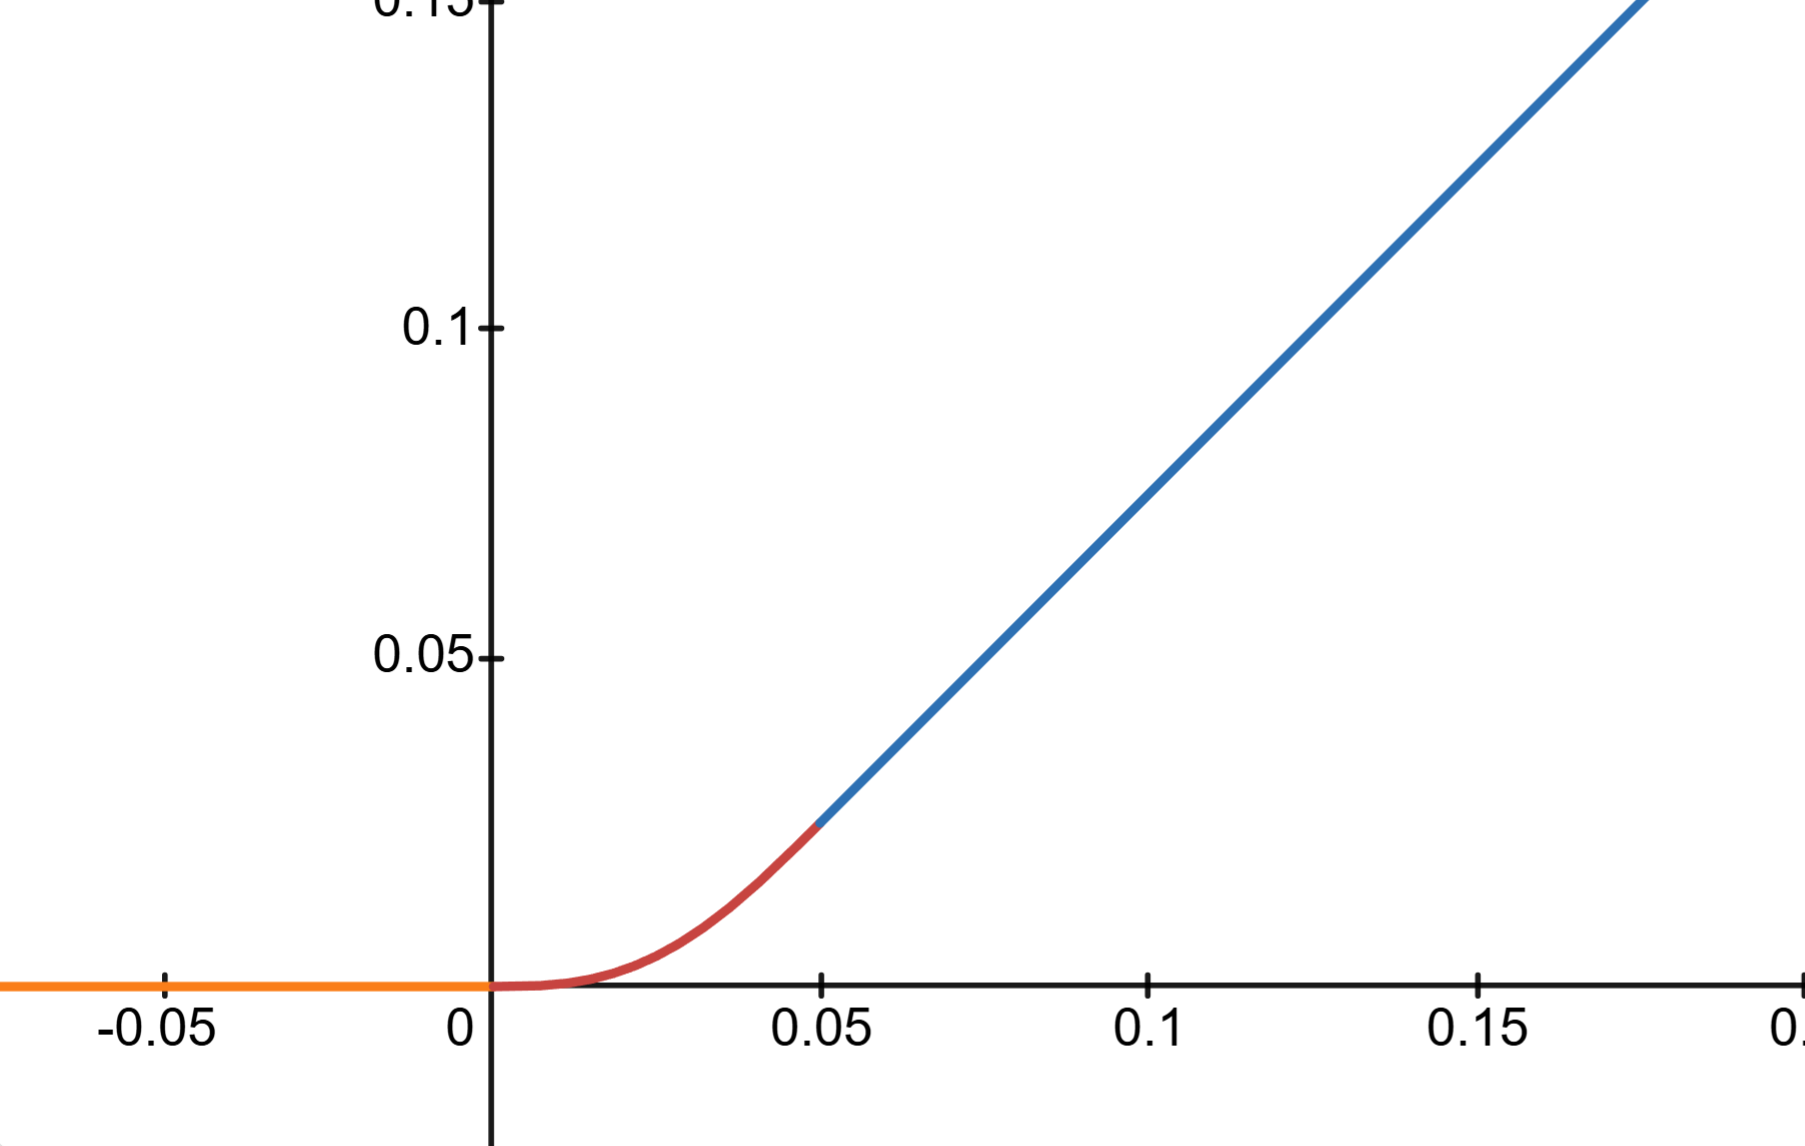
\includegraphics[width=0.8\textwidth]{松弛函数.png}
			\caption{松弛函数}
			\label{fig:松弛函数}
		\end{figure}
		\begin{figure}[!ht]
			\centering
			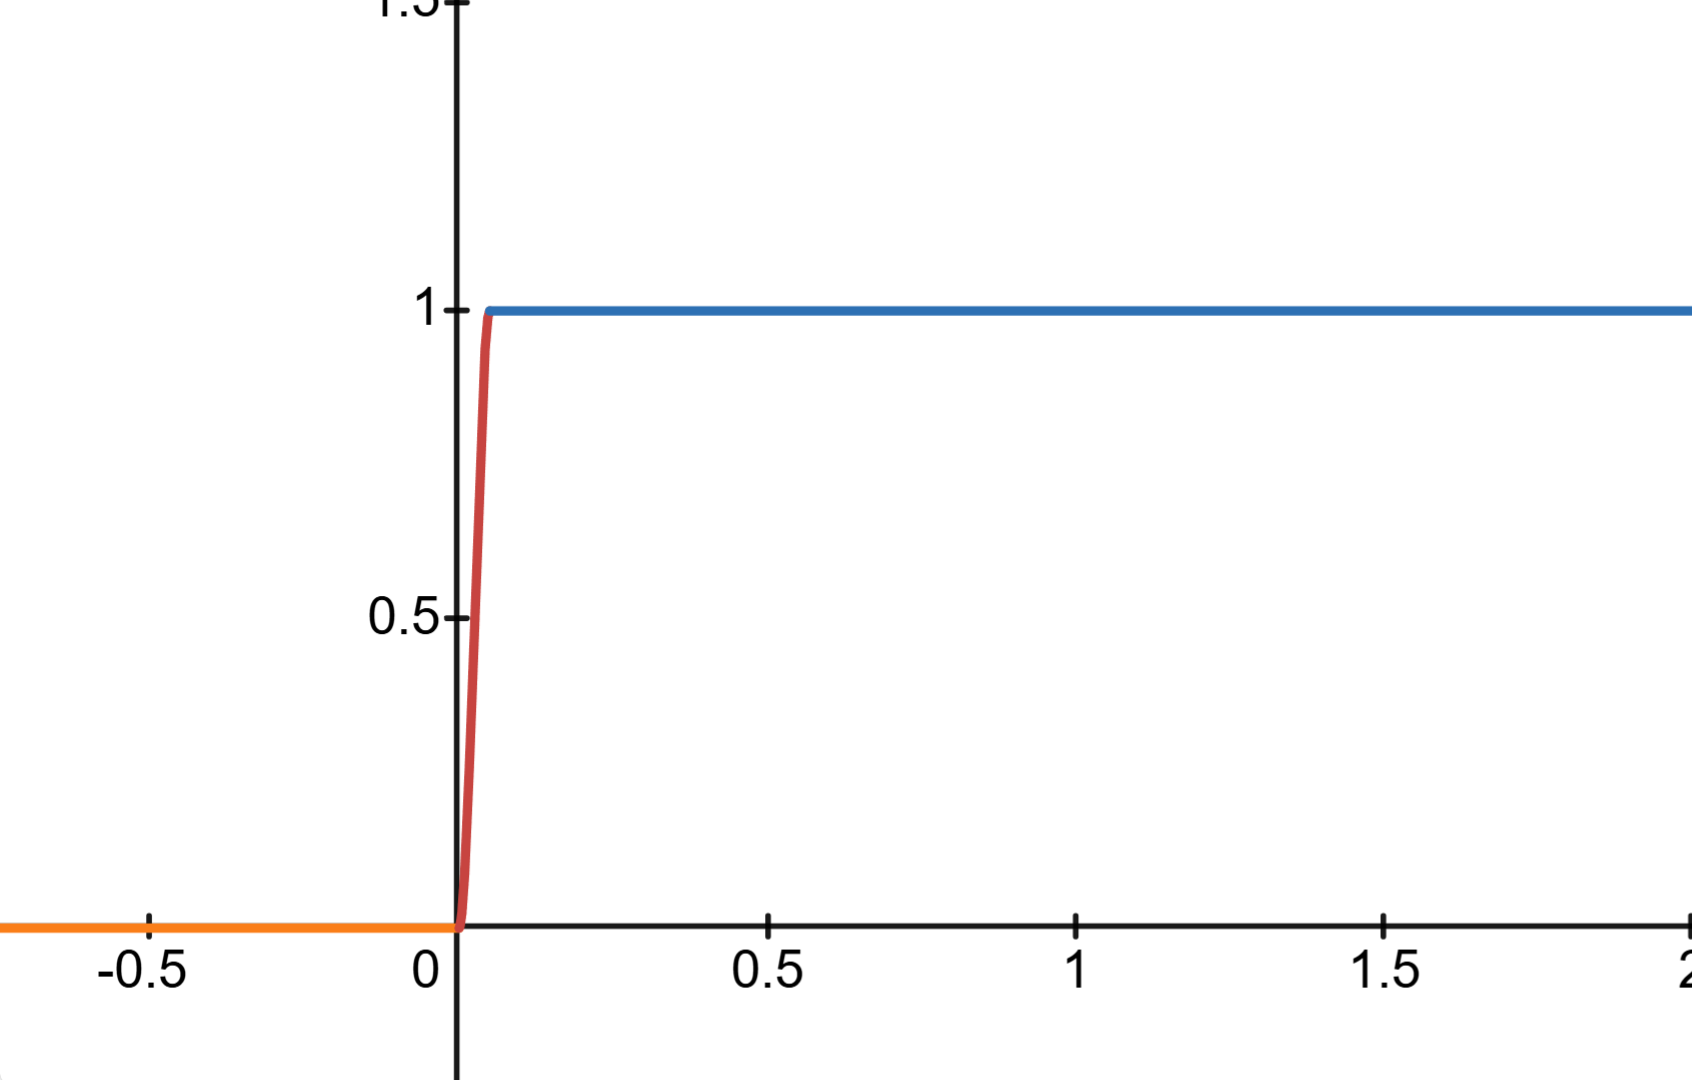
\includegraphics[width=0.8\textwidth]{松弛导数.png}
			\caption{松弛导数}
			\label{fig:松弛导数}
		\end{figure}
		我们设置的a=0.05。可以看出这个函数在x的负半轴的值为0,也就意味着不等式约束的代价为0。在0<x<=a时代价以一个四次函数上升,越靠近原点代价越小。当x>a时代价值以斜率为1直线上升。另外这个分段函数还有非常好的一个特性,在定义域上市C2微分同胚的。这就意味着它的梯度和Hessian矩阵是完全连续的,在优化时我们不必考虑额外的光滑函数。
		综上,问题被化简成了一个无约束的优化问题:
		\begin{equation}
			\begin{aligned}
				\min\text{\ }J( q ) \ =\ \sum_{i=1}^N{\sum_{j=1}^{m_i}{S( -k_m-k_{ij} ) +S( -k_m+k_{ij} ) +S( A_ip_{ij}-b_i )}}
			\end{aligned}
		\end{equation}
		利用矩阵求导的链式法则我们可以求得各个部分的梯度信息,需要指出的是我们矩阵求导遵循分母布局。
		\begin{equation}
			\begin{aligned}
				\frac{\partial S( -k_m-k_{ij} )}{\partial c_i}&=-( \frac{\partial \dot{p}_{ij}}{\partial c_i}\frac{\partial k_{ij}}{\partial \dot{p}_{ij}}+\frac{\partial \ddot{p}_{ij}}{\partial c_i}\frac{\partial k_{ij}}{\partial \ddot{p}_{ij}} ) S^{'} ( -k_m-k_{ij} ) ,\\
				\frac{\partial S( -k_m+k_{ij} )}{\partial c_i}&=( \frac{\partial \dot{p}_{ij}}{\partial c_i}\frac{\partial k_{ij}}{\partial \dot{p}_{ij}}+\frac{\partial \ddot{p}_{ij}}{\partial c_i}\frac{\partial k_{ij}}{\partial \ddot{p}_{ij}} ) S^{'} ( -k_m+k_{ij} ) \\
				\frac{\partial S( A_ip_{ij}-b_i )}{\partial c_i}&=\frac{\partial p_{ij}}{\partial c_i}A_{i}^{T}S^{'}( A_ip_{ij}-b_i ) 
			\end{aligned}
		\end{equation}
		我们利用上式求出了$J$关于$c$的梯度$\frac{\partial J}{\partial q}=\frac{\partial c}{\partial q}\frac{\partial J}{\partial c}$,于是由$b = Mc$,可以推导出:$\frac{\partial b}{\partial q}M^{-T}=\frac{\partial c}{\partial q}$ ,因此$J$关于$q$的梯度为:
		\begin{equation}
			\frac{\partial J}{\partial q}=\frac{\partial c}{\partial q}\frac{\partial J}{\partial c}
		\end{equation}
		
		
		\subsection{优化结果的分析}
		通过上一小节我们推出了路径优化问题的代价函数和梯度信息,这是很关键的。求解无约束优化问题的优化方法有很多,例如最速下降法、牛顿法、共轭梯度法等。对于一般的优化算法而言总体上可以分为两类,一类是基于一阶信息的梯度法,另一类是基于二阶信息的牛顿法。牛顿法除了需要提供代价函数的梯度信息以外,还需要提供代价函数的Hessian矩阵。对于复杂优化问题而言解析计算Hessian是极为复杂的。综合众多因素我们选择使用lbfgs优化算法最为本优化问题的优化求解算法。
		LBFGS算法作为一种高效的拟牛顿优化方法,在优化过程中会不断地迭代逼近出一个Hessian矩阵,省去了手动推导的难度。在大规模无约束优化问题中展现出显著的优势。其核心优势在于内存效率和计算效率,仅存储最近的迭代信息,有效处理高维问题,同时快速收敛于最优解。LBFGS算法的适用性广泛,覆盖机器学习、统计学和工程优化等多个领域,尤其在大规模数据处理中表现出色。
		由于使用优化的方法生成轨迹,所以我们需要一个快速生成航点的路径规划算法,为我们的优化算法提供软起动初值。我们不关心这个算法是否路径最优,但是它需要以较低的时间复杂度运行,因为我们的优化过程可以带来足够的最优性。下面给出我们算法的伪代码:
		 \begin{algorithm}[H]  
		 	\caption{Global Planning}  
		 	\label{Planning}  
		 	\begin{algorithmic}[1]  
		 		\REQUIRE  
		 		$\mathbf{p_{start}},\mathbf{p_{end}},\mathbf{map}$
		 		\ENSURE  
		 		$\mathbf{path}$
		 		\STATE $\hat{path} \leftarrow RRTConnect(\mathbf{p_{start}},\mathbf{p_{end}},\mathbf{map})$
		 		\STATE $cors \leftarrow getCorridor(\mathbf{map},\hat{path})$
		 		\STATE $cons \leftarrow getConstraint(\kappa_{min,max},cors)$
		 		\STATE $costFcn \leftarrow getCost(cons)$
		 		\STATE $grad \leftarrow getGrad(cons)$ \\
		 		\RETURN $\mathbf{path} \leftarrow \mathbf{lbfgs}(costFcn,grad)$
		 	\end{algorithmic}  
		 \end{algorithm}
		 在这里我们推荐使用RRTConnect或者JPS算法,这两者都具有快速生成路径的能力。以下介绍的所有例子都是用RRTConnect生成路径。区别于传统的RRT算法,RRTConnect同时从起点和终点搜索路径,可以显著提高搜索的效率,减少搜索的次数。
		 \begin{figure}[!ht]
		 	\centering
		 	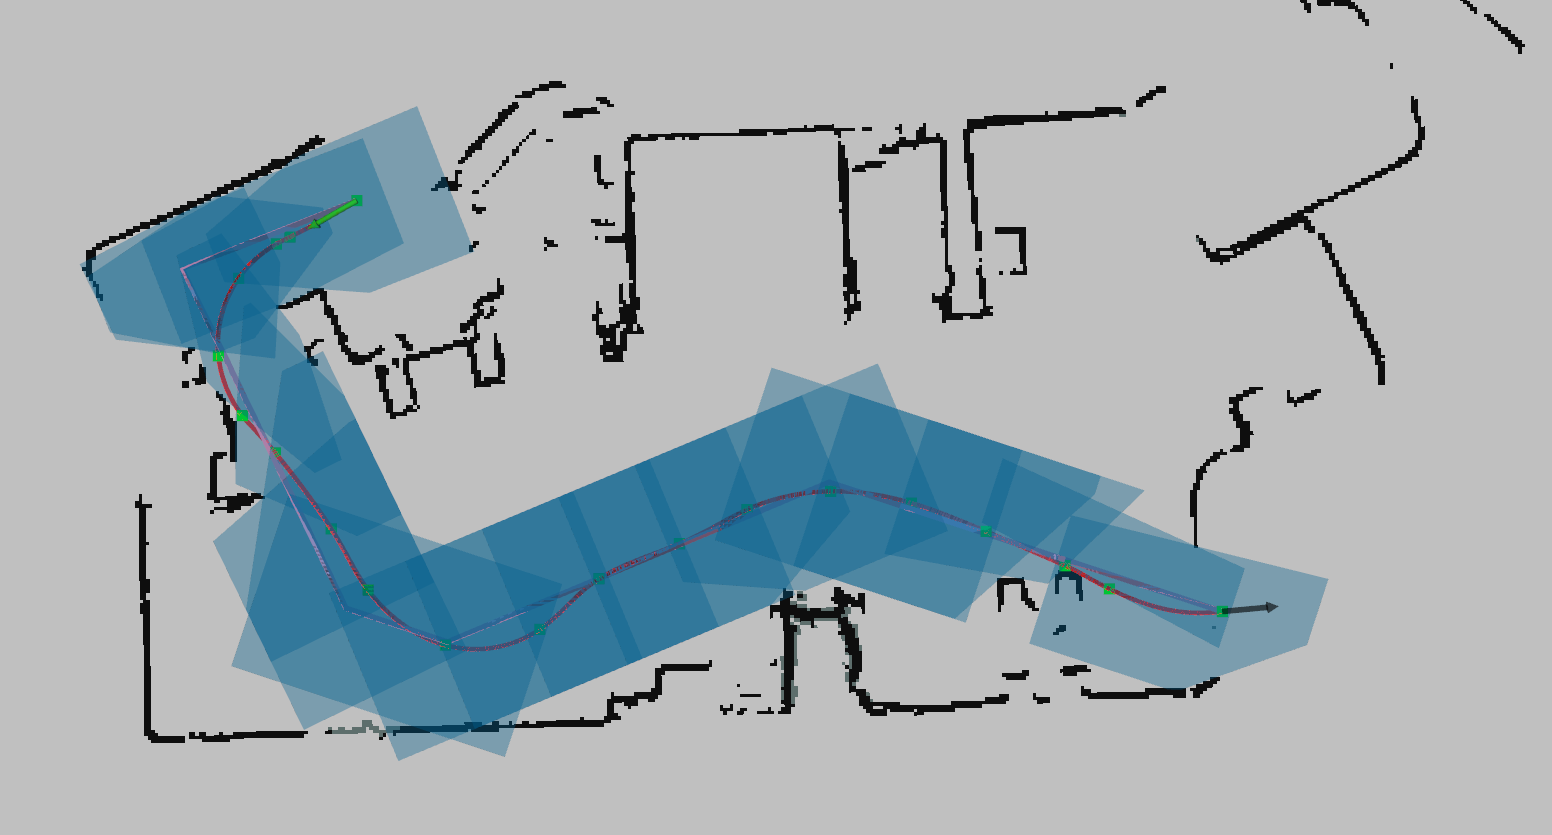
\includegraphics[width=0.8\textwidth]{单轨迹2.png}
		 	\caption{单轨迹2}
		 	\label{fig:单轨迹2}
		 \end{figure}
		 图。。。。是的算法运行的仿真,其中浅紫色那条路径是RRTConnect搜索出的初始路径,他在全局范围内是无碰撞的。沿着初始路径我们生成了如图蓝色的安全走廊,用来表示路径周围的FreeSpace。绿色的点是优化后的航点。红色的是我们优化之后的轨迹,可以看出它严格符合事先给出的曲率约束,并且在完全处于安全走廊内。
		
	\section{多阶段全局轨迹规划案例}
	在上一节中我们描述了一个完整的全局轨迹规划算法,可以完成一个点对点的路径规划问题。对于一些更加复杂的场景,例如码头搬运、舱体清卸、矿山运料等多种复杂的工况下,铰接车需要依次去往各个区域规定完成卸货。这样的场景往往需要面向任务设计一个框架。因为这些场景需要更灵活的运动模式,例如倒车。这一节我们将针对码头搬运场景设计一个周期性的规划流程。
	\begin{figure}[!ht]
		\centering
		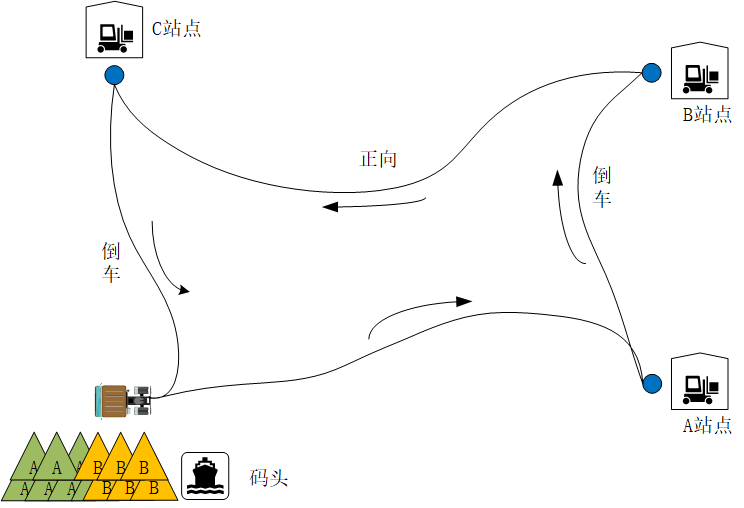
\includegraphics[width=0.8\textwidth]{全局规划.png}
		\caption{全局规划}
		\label{fig:全局规划}
	\end{figure}
		\subsection{多阶段规划的问题描述}
		考虑【如图】的搬运问题,我们需要铰接车从起点码头装货完成去往A点进行卸货,然后去往B点,再去C点,最后回到码头重新装货。这个搬运周期一共需要四次规划,且搬运过程中由于环境等因素规划过程需要倒车。
		\subsection{航点过渡策略}
		在整个规划周期中铰接车一共需要经过四个航点,分别为码头、A站点、B站点和C站点。在整个过程中受到路径受到两个方面的限制。第一,每一段轨迹的起点的切线方向必须和铰接车保持一致,这可以由曲率约束所保证。第二,如果在航点处需要求车辆发生换向,则换向后的轨迹的航向和换向前应该相反。 
		
		A、轨迹起点和初始位姿一致性保证
		由于我们使用minco对x和y方向分开规划,所以铰接车的初始位姿要同时作用在x和y两个方向上。记初始的姿态为$\theta_s$ ,由运动学模型我们可以求得:
		\begin{equation}
			v_{sx}=v_scos\theta _s\\
			v_{sy}=v_ssin\theta _s
		\end{equation}
		对于初始速度$v_s$不为零的情况,$v_{sx},v_{sy}$都不等于零,我们带入优化问题就可以直接保证车辆初始朝向和轨迹的起点切向在一条直线上。但是当$v_{s}=0$时,推出$v_{sx}=0,v_{sy}=0$。此时用平坦模型计算$\theta_s$:
		\begin{equation}
			\theta_s=\text{atan}2\left( v_{sy},v_{sx} \right) =\text{atan}2\left( 0,0 \right) 
		\end{equation}
		我们发现其实当$v_{s}=0$时曲线的切线方向是没有定义的,这是一个奇异点。为了处理这种奇异情况,我们给当$v_{s}$加上一个微小正量保证它的有效性:
		\begin{equation}
			\begin{aligned}
			v_{sx}&=\left( v_s+\epsilon \right) cos\theta_s\\
			v_{sy}&=\left( v_s+\epsilon \right) sin\theta_s,0<\epsilon <1e-5.
			\end{aligned}
		\end{equation}
		这样就可以保证车辆的起点朝向施加在轨迹上,同样由于$\epsilon$是一个极小量,它几乎不会影响轨迹起点的初始速度。对于终点的处理方法和起点一样。
		
		B、航点的换向处理
		
		在中间航点处的是否换向包含两种情况,一种是航点前的车辆运动方向和航点后运动方向相同,则不需要换向。另一种是航点前的车辆运动方向和航点后运动方向相反,则需要换向,此航点也被称为换向点。
		\begin{figure}[!ht]
			\centering
			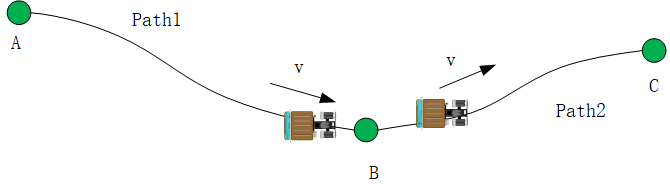
\includegraphics[width=0.8\textwidth]{换向1.png}
			\caption{换向1}
			\label{fig:换向1}
		\end{figure}
		\begin{figure}[!ht]
			\centering
			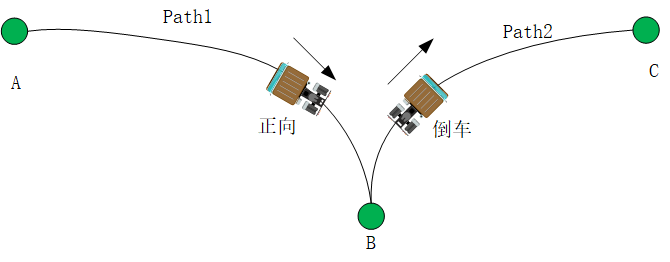
\includegraphics[width=0.8\textwidth]{换向2.png}
			\caption{换向2}
			\label{fig:换向2}
		\end{figure}
		图【】是表示的是车正向行驶穿越航点的情况,经过航点时不用倒车。我们在规划AB段路径时B点作为终点,在规划BC段路径时B点作为起点车辆的运动方向和车辆的朝向相同。图【】是表示的是车正向行驶到达航点,再反向倒车。与图【】不同的是,在规划BC段路径时B点作为起点车辆的运动方向和车辆的朝向相反,而AB段相同,因此规划BC段时B点作为起点需要反向。
		\subsection{规划结果展示}
		下面是我们算法在码头地图中的多阶段规划例子:
		\begin{figure}[!ht]
			\centering
			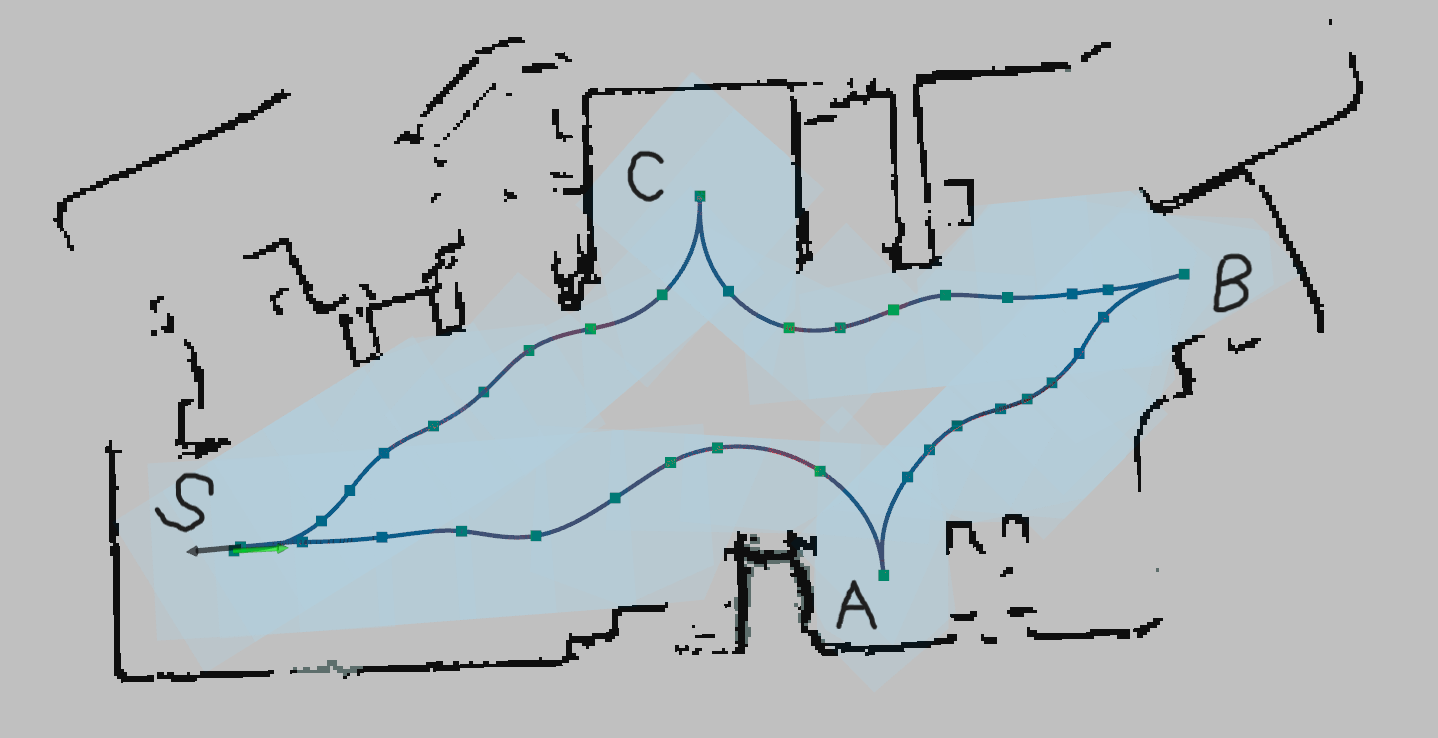
\includegraphics[width=0.8\textwidth]{多阶段轨迹s.png}
			\caption{多阶段轨迹s}
			\label{fig:多阶段轨迹s}
		\end{figure}
	\section{本章总结}
	在这节中我们介绍了铰接车的微分平坦模型,并使用minco参数化了我们轨迹的形式。然后我们分析了轨迹的安全约束和曲率约束。最后我们建立了一个点对点的规划问题,并给出了一个码头搬运的小案例。
	
	
	\chapter{基于安全走廊的无人铰接车局部规划方法}
	在这一章中我们主要介绍一种基于安全走廊的时空联合轨迹规划方法,这种方法采用最优控制(Optimal Control)的框架对问题建模。第一节中我们将对铰接车外观做一个通用性的建模,可以有效加强碰撞检测的速度。第二节中介绍针对于铰接车改进的Hybrid A*算法,它将用于我们轨迹规划算法的热启动。第三节介绍规划问题中涉及到的所有约束并进行处理。第四节我们对优化问题进行求解。
	\section{铰接车的一般性结构建模}
	为了保持优化问题的凸性,将车辆底盘形状建模为两个矩形的连接,从而将装载机的避障问题转化为多边形几何碰撞问题。车辆形状分为前轴和后轴两部分,共由九个顶点A,B,C,…,H和O1。这些顶点在车辆车身坐标系中的表示如下:
	\begin{figure}[!ht]
		\centering
		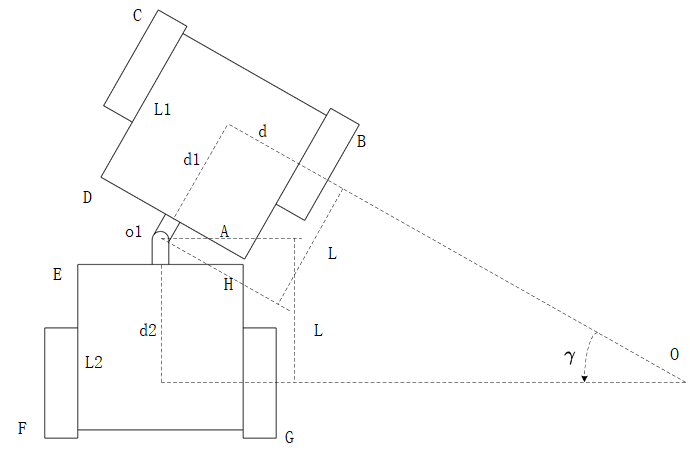
\includegraphics[width=0.8\textwidth]{ppi.png}
		\caption{ppi}
		\label{fig:ppi}
	\end{figure}
	与动学模型相一致,我们选取前后中点作为参考点$(x_f,y_f)$,沿着车体方向作为x轴正方向。则A,B,C,…,H和O1的相对坐标可以表示为:
	\begin{equation}
		\begin{aligned}
			l_{A}^{T}&= -d_1,-width/2 ) ,l_{B}^{T}= L_1-L,-width/2 ) ,\\
			l_{C}^{T}&= L_1-L,width/2 ) ,l_{D}^{T}= -d_1,width/2 ) ,\\
			l_{E}^{T}&= d_2-L,width/2 ) ,l_{F}^{T}= -L_2,width/2 ) ,\\
			l_{G}^{T}&= -L_2,-width/2 ) ,l_{H}^{T}= d_2-L,-width/2 ) ,\\
			l_{O_1}^{T}&= -L,0 ) .\\
		\end{aligned}
	\end{equation}
	其中,lA,lB,lC,lD,lo1表示相对于底盘前桥坐标系下的坐标。lE,lF,lG,lH是相对于铰接点坐标系下的坐标。在世界坐标系中,坐标可以表示为旋转矩阵$R_\theta$和平移向量$\sigma$的组合。因此,根据(6),前轴的顶点集表示如下
	\begin{equation}
	\begin{aligned}
		\varepsilon_f = \left\{ p_f \in \mathbb{R}^2 \mid p_f=R_\theta l_f+\sigma,  f = A,B,C,D \right\},
	\end{aligned} 
	\end{equation}
	
	在这里$\sigma$表示前轴参考点坐标,表示为$\sigma=(x_f,y_f)$。在从世界坐标系到铰接点坐标系的变换中,还涉及到车身坐标系,需要应用旋转矩阵$R_\theta$和$R_\gamma$。平移向量由世界坐标系中的铰接点给出,记为$\sigma_1$。在(5)中,模型各点的坐标变换可表示为:
	\begin{equation}
		\begin{aligned}
			&\left\{\begin{matrix}
				p_r=R_\gamma R_\theta l_b+\sigma_1\\
				\sigma_1=R_\theta l_{O_1}+\sigma
			\end{matrix}\right.   \Longrightarrow \varepsilon_r ,\\
			&\varepsilon_r = \left\{ p_r \in \mathbb{R}^2 \mid p_r=R_\gamma R_\theta l_r+R_\theta l_{O_1}+\sigma,  \right\} ,\\
			&r = E,F,G,H.
		\end{aligned}
	\end{equation}
	
	\section{铰接车Hybrid A*算法的创新改进}
	在大规模优化问题中,影响求解质量的主要因素往往不是问题或约束的非线性特性,而是问题是否具备凸性。遗憾的是,大多数非线性规划问题都不具备凸性,只有少数问题能够通过对偶方法、变换等手段转化为凸优化问题。直接求解这类问题时,常常会陷入局部最优解,难以保证找到全局最优解。然而,对于这些非凸问题,我们依然可以采用其他思路,找到最优解或一个较为理想的解。关键在于,尽管问题本身无法严格保证非凸性,我们仍然可以使用一些全局最优算法,通过寻找一个接近最优的初值来确保其位于全局最优解所在的凸空间内。接下来,优化算法可以沿着这个初值在局部凸空间内展开迭代,最终找到最优解。
	例如,在百度Apollo的轨迹规划中,轨迹优化基元采用了多项式形式,通过优化控制点来生成满足要求的轨迹。在此过程中,控制点的初值是通过动态规划搜索得到的。动态规划的作用在于,通过对状态空间的逐步分解,找到一个合理的凸空间,使得优化算法能够高效地进行局部最优解的搜索。
	Hybrid A star算法首次应用于2007年DAPPA城市挑战赛,并由Dolgov等人提出。与传统的A star算法不同,Hybrid A star算法在三维空间中进行搜索,且在搜索过程中,邻居节点的拓展是通过动力学方程的前向推演来实现的。然而,传统的Hybrid A star算法是基于$x-y-\theta$三维空间进行搜索的,这使得它并不适用于铰接车模型。铰接车由于其具有较为复杂的非线性运动特性,因此直接应用传统的Hybrid A*算法会面临难以满足约束条件和路径质量不高的问题。
	为了使Hybrid A star算法能够适应铰接车的路径规划问题,本节将提出一种创新性的改进方法。具体来说,我们将修改Hybrid A算法中的邻居节点拓展策略,结合铰接车的运动学特性,改进算法的搜索策略,以便更好地在铰接车的状态空间中找到一个次优的初解。该初解将在后续的优化过程中作为起点,进一步引导算法沿着合适的方向优化,最终得到一个更加符合实际需求的路径。通过这种方式,我们能够克服传统Hybrid A*算法的局限性,为铰接车路径规划提供更为高效和精准的解决方案。
		\subsection{节点拓展策略改进}
		铰接车的位形(configuration)传统汽车有显著差异,其位形不仅依赖于车辆的位置和方向$(x,y,\theta)$,还受到铰接角$(gamma)$的影响。假设铰接车当前的状态为$x_0(x,y,\theta,\gamma)$,一般的hybrid算法将控制区间$[-v_{max},v_{max}]$和$[-\omega_{max},\omega_{max}]$进行离散化。并从当前状态$x_0$开始以输入采样值$[v,\omega]$在$\Delta_t$时间内进行运动学推演得到下一个状态,运动学推演见公式a,推演过程如图a。
		\begin{figure}[!ht]
			\centering
			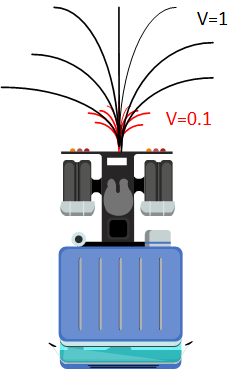
\includegraphics[width=0.5\textwidth]{hybrid采样.png}
			\caption{hybrid采样}
			\label{fig:hybrid采样}
		\end{figure}
		图a只简单列出了速度为0.1和1的情况。可以看出这种采样方式在$|v|$很小时,不管$\omega$为多少,所积分出来的轨迹都会聚在一起。如图a中的红色轨迹有短又聚合,并没有充分的去探索周围空间。这是很浪费计算资源且没有必要的。第二,由于系统的输入是二维$(v,omega)$,所以算法的时间复杂度是$O(N^2)$。下面我将针对节点采样进行改进,可以有效解决采样出来的轨迹聚合的问题,并以$O(N)$时间复杂度完成探索,某种意义上这也是一种轨迹的剪枝策略。 
		首先我们为了降低计算的复杂度,我们只使用铰接车的静态转向模型,系统的输入为$(v,\gamma_u)$。我们不再以固定的时间$\Delta_t$进行采样,我们以固定的行驶路程$\Delta_s$采样,于是系统的输入就只有$\gamma_u$。这样做的本质是只在路径几何层面考虑规划问题。运动学推演方程如下:
		\begin{equation}
			\begin{aligned}
				\left[ \begin{array}{c}
					x_{k+1}\\
					y_{k+1}\\
					\theta _{k+1}\\
					\gamma _{k+1}\\
				\end{array} \right] =\left[ \begin{array}{c}
					x_k+\Delta s\cdot cos\theta _k\\
					y_k+\Delta s\cdot sin\theta _k\\
					\theta _k+\frac{\Delta s}{L}\cdot tan (\gamma _{uk}/2 )\\
					\gamma _{uk}\\
				\end{array} \right] 
			\end{aligned}
		\end{equation}
		其中$\Delta_s$是采样的路径步长,$(x,y,theta,gamma)$是铰接车的位形空间状态变量。$\Delta_s$等于2m的推演过程如图b。
		\begin{figure}[!ht]
			\centering
			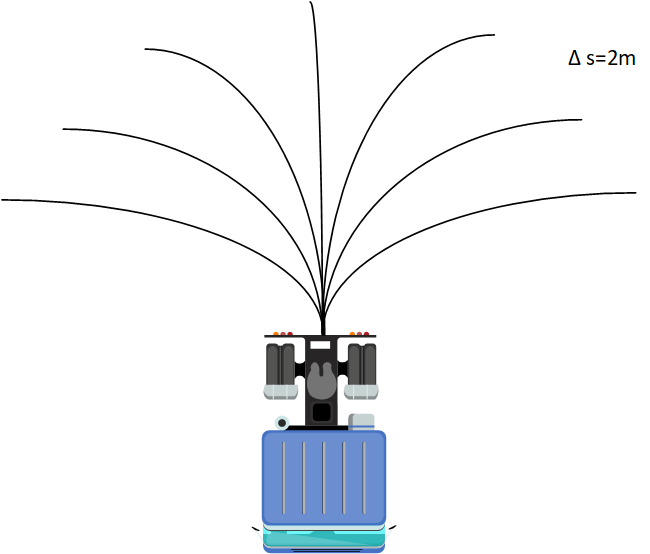
\includegraphics[width=0.8\textwidth]{hybrid采样改进剪枝.png}
			\caption{hybrid采样改进剪枝}
			\label{fig:hybrid采样改进剪枝}
		\end{figure}
		可以看出相对于图a来说采用图b的方式可以大大降低时间复杂度。本质上这其实也是v为固定常数时的特殊情况。
		此外为了加速搜索,hybridA在搜索过程中还引入了Reeds-Shepp曲线,进一步提高搜索效率。Reeds-Shepp曲线生成算法由J.A. Reeds和L.A. Shepp于1990年提出,是一种用于求解二维平面中任意始末位姿之间最短路径的算法。该算法的核心思想是通过分析并归纳所有可能的路径类型,将最短路径的构造问题简化为48种不同的情况,并且对每种情况进行了枚举,涵盖了圆弧和直线段的各种排列组合方式。因此,Reeds-Shepp曲线可以为无障碍情况下的最短路径提供解析表达式,并能够快速地构造出符合运动学约束的可行路径。Reeds-Shepp曲线特别适用于涉及到转向半径约束的路径规划问题,尤其是在移动机器人和自动驾驶领域中,其广泛应用于生成车辆的路径规划。该算法通过考虑车辆的运动学约束(如最小转弯半径),能够有效地找到从起点到终点的最短路径,并确保路径是可行的,符合实际的转向和行驶要求。值得指出的是,Reeds-Shepp曲线在hybridA搜索的最后一步具有加速收敛到终点的效果。
		\subsection{代价函数设计}
		HybridA算法在进行节点的扩展时,会从采样出来的节点中选出代价最低的一个节点作为下一个扩展节点。HybridA算法的代价函数f分为累积代g和启发式函数代价h两个部分。其中累积代价g表征着起点到当前节点的路程代价,启发式代价h表征当前节点到终点的代价。值得注意的是一般当前点到终点的最小代价是未知的,所以理论上启发式函数h设计的越靠近最优代价则搜索效果越好。
		
		在上一小节中我们的采样策略的输入变量是$\gamma_u$,由于上一时刻的采样和这一时刻独立,所以可能出现$\Delta_{\gamma}$过大的情况,也就是铰接角突变问题,这对于下层控制是不利的。所以我们在代价函数中必须含有$\Delta_{\gamma}$项使得铰接角变化率尽量小,我们称之为转向惩罚。因此我们将累积代价设计为:
		\begin{equation}
			\begin{aligned}
				g_k=g_{k-1}+ x_k-x_{k-1} ) ^2+ y_k-y_{k-1} ) ^2+ \gamma _{uk}-\gamma _{u k-1 )} ) ^2
			\end{aligned}
		\end{equation}
		启发式代价函数h记录当前节点到终点的估计代价,hybridA算法的启发式代价一般分为两个部分:非完整约束启发式代价$h_{nonh}$和避障启发式代价$h_{collision}$。其中非完整约束代价$h_{nonh}$是仅仅在考虑车辆有转弯半径且不考虑障碍物的情况下的代价,通常可以直接由Reeds-Shepp闭式算出。避障启发式代价$h_{collision}$则是仅考虑避障时的代价,这里我们使用无穷范数作为避障启发式代价。
		\begin{equation}
			\begin{aligned}
				g_k=g_{k-1}+ x_k-x_{k-1} ) ^2+ y_k-y_{k-1} ) ^2+ \gamma _{uk}-\gamma _{u k-1 )} ) ^2
			\end{aligned}
		\end{equation}
		\subsection{碰撞检测算法设计}
		在碰撞检测算法的设计中,我们通过检查车辆几何模型与栅格地图的是否有重叠来判断路径可行性,其核心原理基于车辆位姿变换与离散化障碍物检测。首先,算法利用旋转矩阵将车辆初始轮廓坐标变换到全局坐标系下,计算各顶点坐标后转换为地图栅格索引,以便在栅格地图中查询索引处是否由障碍物。随后,对车辆轮廓边进行线段离散化检测。如图c所示,采用Bresenham算法遍历每条边的栅格路径,若任一栅格为障碍物或超出地图边界,则判定为碰撞。在路径搜索过程中,该模块嵌入节点扩展和Reeds-Shepp曲线连接阶段,逐段验证候选路径的安全性。其优势在于计算效率高且与栅格地图兼容性强,但受限于离散化误差可能忽略细小障碍物,且仅适用于静态环境。图c中左图为家铰接车在空间中安全的场景,右图则是发生碰撞的场景,其中红色栅格是车体轮廓和障碍物栅格重叠的区域。
		\begin{figure}[!ht]
			\centering
			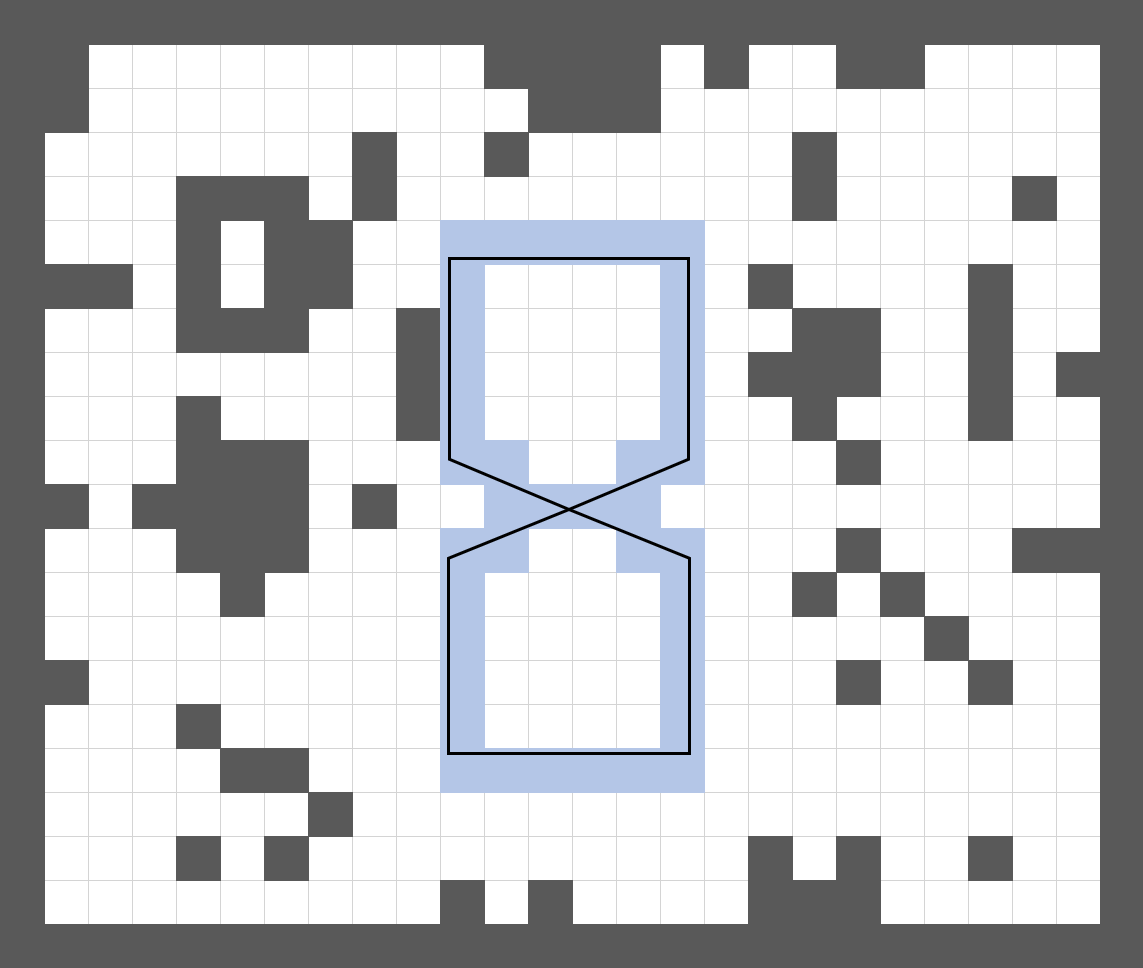
\includegraphics[width=0.8\textwidth]{bresham_free.png}
			\caption{breshamfree}
			\label{fig:bresham_free}
		\end{figure}
		
		\begin{figure}[!ht]
			\centering
			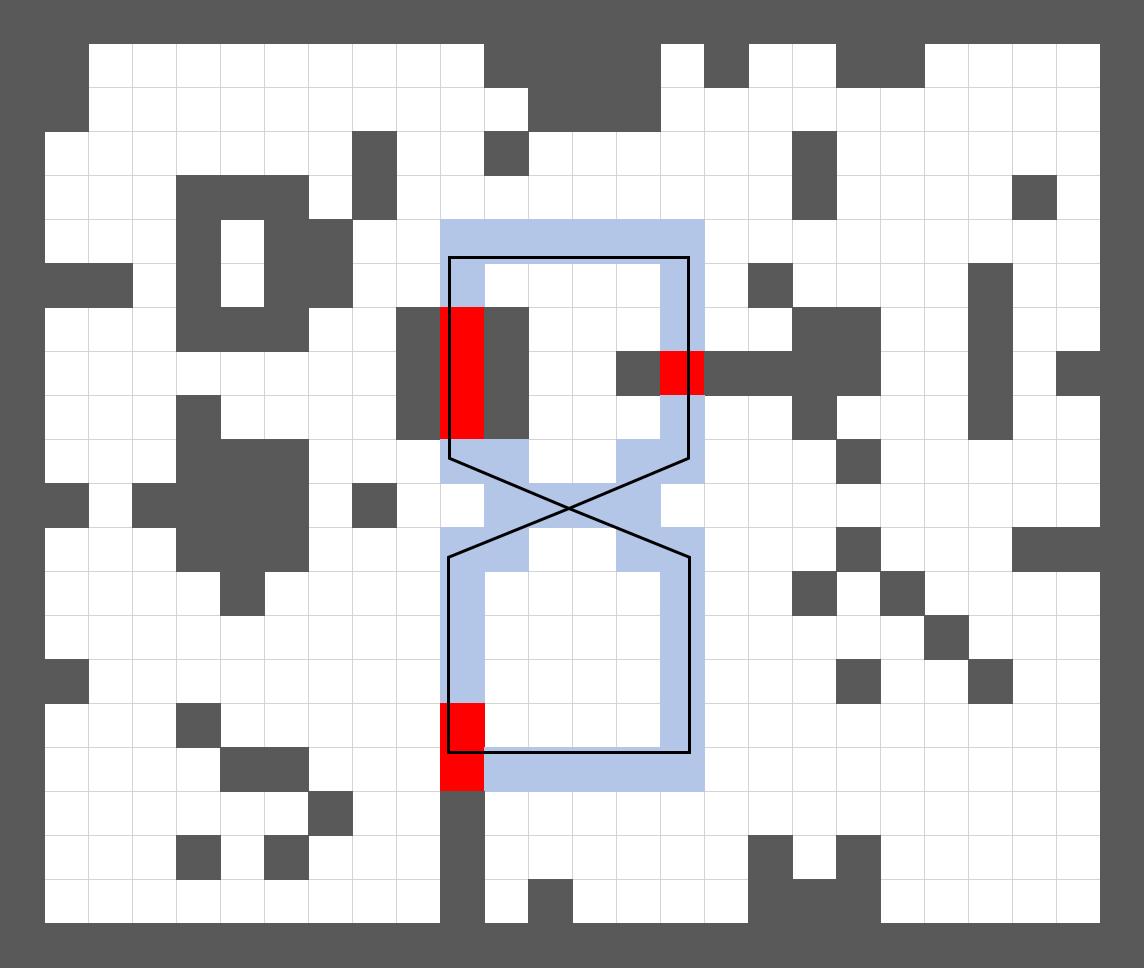
\includegraphics[width=0.8\textwidth]{bresham_colli.png}
			\caption{breshamcolli}
			\label{fig:bresham_colli}
		\end{figure}
	\section{基于NMPC和安全走廊的轨迹规划}
	在4.2节中我们针对铰接车对hybridAstar算法进行了改进,它将作为我们轨迹规划的热启动算法。本节中将介绍如何构建一个基于NMPC的轨迹规划算法,这是一个典型的OCP最优控制框架。
		\subsection{NMPC问题构建}
		铰接式车辆运动规划的最优控制问题可以表示为其一般形式,包括成本函数以及多个等式或不等式约束。与典型的优化问题不同,基于最优控制的轨迹规划还受到一组动态微分方程的约束。一般能耗和时间最优的代价函数定义如下:
		\begin{equation}
			\begin{aligned}
				J(x(t),u(t)) &= \int_{t_0}^{t_f}
				\left\| u(t)\right\|^2dt +w_t*\left\|t_f-t_0\right\|^2,    \\
				\left\|u(t)\right\|^2&=w_{uj}*\left\|jerk(t)\right\|^2+w_{uw}*\left\|\omega\right\|^2.
			\end{aligned} 
		\end{equation}
		其中 $w_t$、$w_{uj}$ 和 $w_{uw}$ 分别为时间代价权重、舒适度代价权重和铰接角能耗代价权重。$\left\|u(t)\right\|^2$ 用作输入能量消耗的度量,而 $\|t_f- t_0\|^2$ 确保时间持续时间的最优性,其中 $t_f$ 和 $t_0$ 分别为结束时间和开始时间。然后这个轨迹优化问题表示为:
		\begin{equation}
			\begin{aligned}
				&\left[x^*(t),u^*(t)\right] = minimize\ J(x(t),u(t)),\\      
				&s.t.\ \dot x(t)-f(x(t),u(t))=0,\\
				&x_l \leq x(t) \leq x_u, u_l \leq u(t) \leq u_u,t\in \left[0,t_f\right],\\
				&x(t_0)=x_{start},x(t_f)=x_{goal}.\label{4}
			\end{aligned}   
		\end{equation}
		在公式()的约束中,$\dot x(t)-f(x(t),u(t))=0$表示运动方程约束,保证优化问题中轨迹的平滑性。变量$x_l$和$x_u$表示状态变量的下界和上界,$u_l$和$u_u$表示控制变量的下界和上界。此外,$x_{start}$和$x_{goal}$分别对应规划问题的起点和终点。
		\subsection{运动学约束}
		如公式,在第二章中我们介绍了铰接车的运动学模型。这个运动学模型的状态量为x,y,theta,gamma,受到微分方程的约束这些变量是天然连续的。系统的输入为速度v和铰接角速度omega,他们并没有受到微分方程的约束,这意味着v和omega在优化过程中直接作为优化变量是会突变的。这对于下层控制来说是不利的。为了解决这个问题,我们为系统引入高阶信息的连续性,假设系统的输入为jerk(加加速度或者舒适度)和omega。模型可以进一步写为:
		\begin{equation}
			\begin{aligned}
				\dot{x}=f x,u ) \Longrightarrow \frac{d}{dt}\left[ \begin{array}{c}
					x_f\\
					y_f\\
					\theta\\
					\gamma\\
					v\\
					a\\
				\end{array} \right] =\left[ \begin{array}{c}
					vcos\theta\\
					vsin\theta\\
					vtan \gamma /2 ) /L+\omega / cos\gamma +1 )\\
					\omega\\
					a\\
					jerk\\
				\end{array} \right] 
			\end{aligned}   
		\end{equation}
		在这里 $x=\left[ x_f,y_f,\theta,\gamma,v,a \right]^T$ 为状态向量,分别表示前轴中点位置、航向角、铰接角、速度、加速度。输入向量由 $u=\left[jerk,w\right]^T$ 给出,其中 $jerk$ 为前轴中点加加速度(舒适度),$w$ 为铰接角速度。
		对于上述运动学方程我们对其进行离散化,采用一阶离散运动学模型,可表示为:
		\begin{equation}
			\begin{aligned}
				x k ) =x k-1 ) +\Delta t k-1 ) f x k-1 ) ,u k-1 ) ) 
			\end{aligned}   
		\end{equation}
		我们令 \(g_{\text{kin}} = [g_x^T\ g_y^T\ g_\theta^T\ g_\gamma^T\ g_v^T\ g_a^T]^T\),其中每个 \(g\) 对应 \(m = N-1\) 个等式约束。例如:
		\begin{equation}
			\begin{aligned}
				g_{x_f} 0 ) =x_f 1 ) -x_{start}-\Delta t 0 ) \cdot v 0 ) \cos \theta  0 ) ,\\
				g_{x_f} 1 ) =x_f 2 ) -x_f 1 ) -\Delta t 1 ) \cdot v 1 ) \cos \theta  1 ) ,\\
				...\\
				g_{y_f} 0 ) =y_f 1 ) -x_{start}-\Delta t 0 ) \cdot v 0 ) \sin \theta  0 ) ,\\
				g_{y_f} 1 ) =y_f 2 ) -y_f 1 ) -\Delta t 1 ) \cdot v 1 ) \sin \theta  1 ) ,\\
				...
			\end{aligned}   
		\end{equation}
		使用惩罚函数将运动学约束纳入成本函数,表达式如下:
		\begin{equation}
			\mathcal{G}_{kin} = w_{kin}*\left \| g_{kin} \right \|_2^2
		\end{equation}
		梯度为:
		\begin{equation}
			\frac{\partial\mathcal{G}_{kin}}{\partial\xi}=2w_{kin}\cdot\frac{\partial g_{kin}^T}{\partial\xi}\cdot g_{kin}\label{18}
		\end{equation}
		其中 \(\frac{\partial g_{\text{kin}}^T}{\partial \xi}\) 表示所有运动约束向量的雅可比矩阵。假设第 \(i\) 类运动约束关于第 \(j\) 类变量的雅可比矩阵由 \(\psi_{ij} = \frac{\partial g^T_{i}}{\partial \xi_j}\) 给出。我们可以推出:
		\begin{equation}
			\begin{array}{c}
				\frac{\partial g_{k i n}^{T}}{\partial \xi}= \\
				{\left[\begin{array}{cccccc}
						\psi_{E} & 0 & 0 & 0 & 0 & 0 \\
						0 & \psi_{E} & 0 & 0 & 0 & 0 \\
						-\psi_{x \theta} & -\psi_{y \theta} & \psi_{E} & 0 & 0 & 0 \\
						0 & 0 & -\psi_{\theta \gamma} & \psi_{E} & 0 & 0 \\
						-\psi_{x v} & -\psi_{y v} & -\psi_{\theta v} & 0 & \psi_{E} & 0 \\
						0 & 0 & 0 & 0 & -\psi_{v a} & \psi_{E} \\
						0 & 0 & -\psi_{\theta \omega} & -\psi_{\gamma \omega} & 0 & 0 \\
						0 & 0 & 0 & 0 & 0 & -\psi_{\text {ajerk }} \\
						-\psi_{x \Delta t} & -\psi_{y \Delta t} & -\psi_{\theta \Delta t} & -\psi_{\gamma \Delta t} & -\psi_{v \Delta t} & -\psi_{a \Delta t}
					\end{array}\right]}
			\end{array}
		\end{equation}
		其中 $\psi _ = [_{n \times n}, 0_n] - [0_n, E_{n \times n}]$,其中 $E$ 为单位矩阵,且\(\psi_{ij} = \frac{\partial g^T_{i}}{\partial \xi_j}\)。
		\subsection{基于安全走廊的防碰撞约束}
		为了方便表达,我们定义 \([]\) 为逐元素运算符,例如 \([\cdot]\) 表示逐元素乘法,\(S[x]\) 表示对$x$的所有元素进行函数 \(S\)运算 。
		引入惩罚项和松弛函数来处理走廊的不等式约束,得到以下结果,其表达为:
		\begin{equation}
			\mathcal{G}_c =\mathcal{G}_{f}+\mathcal{G}_{r}=w_{c}\cdot \sum_{k=1}^{N-2}\sum_{i=0}^{d-1}(S[g_f(k)] + S[g_r(k)]).\label{20}
		\end{equation}
			其中$d$为矩阵$A_k$的行数。为了确保连续可微性,松弛函数$S(x)$仍然使用第三章中的公式(3-21)。
			把公式(4-15)
		
		\subsection{边界条件}
		\subsection{时间正则化约束}
		\subsection{迭代求解框架}
	\section{本章小结}
	
	

	\chapter{结论}
		论文的结论部分是整个研究的归纳和总结,也是对研究问题的回答和对结果的解释。在这一部分中,研究者应该系统性地总结研究的主要发现,并就这些发现的意义进行讨论。同时,应该指出研究的局限性,并提出未来研究的方向。

		首先,结论部分应该对研究的核心发现进行简要总结,强调这些发现与研究问题之间的关系。然后,研究者需要讨论这些发现的意义,包括对理论、实践或政策的影响,并强调研究的贡献。此外,应该指出研究的局限性,即研究所面临的限制和可能存在的偏差,并提出改进方法。最后,结论部分应该提出未来研究的方向或建议,以便激发读者的兴趣,并为后续研究提供参考。

		总之,结论部分是整个论文的重要组成部分,需要深入总结研究的主要发现,并就这些发现的意义进行深入讨论,同时指出研究的局限性并提出未来研究的方向。

	\reference{ref.bib}

	\customizedappendix{
		%如无附录,可删除此部分内容。
		论文的附录通常包括一些额外的材料,用于补充和支持主体文本,但不适合直接放在正文中。以下是一些可能包含在附录中的内容。
		
		\begin{align}
			\theta&=\omega t\notag\\
			a&=\cos\theta \label{eq:appendix1_a}\\
			b&=\sin\theta \label{eq:appendix1_b}\\
			a^2+b^2&=1
			\label{eq:appendix1_a^2+b^2}
		\end{align}
		
		\begin{subequations}
			\label{eq2:appendix1_identity_a_b}
			\begin{align}
				\theta&=\omega t\notag\\
				a&=\cos\theta \label{eq2:appendix1_a}\\
				b&=\sin\theta \label{eq2:appendix1_b}\\
				a^2+b^2&=1
				\label{eq2:appendix1_a^2+b^2}
			\end{align}
		\end{subequations}
	}

	\customizedappendix{
		%如无附录,可删除此部分内容。
		论文的附录通常包括一些额外的材料,用于补充和支持主体文本,但不适合直接放在正文中。以下是一些可能包含在附录中的内容。
		
		\begin{align}
			\theta&=\omega t\notag\\
			a&=\cos\theta \label{eq:appendix2_a}\\
			b&=\sin\theta \label{eq:appendix2_b}\\
			a^2+b^2&=1
			\label{eq:appendix2_a^2+b^2}
		\end{align}
		
		\begin{subequations}
			\label{eq2:appendix2_identity_a_b}
			\begin{align}
				\theta&=\omega t\notag\\
				a&=\cos\theta \label{eq2:appendix2_a}\\
				b&=\sin\theta \label{eq2:appendix2_b}\\
				a^2+b^2&=1
				\label{eq2:appendix2_a^2+b^2}
			\end{align}
		\end{subequations}
	}


	\achievement{
		{\vspace{-0.1em}\noindent\textbf{\songtib\zihao{-4} 1.\enspace 发表的学术论文}\vspace{-0.41em}}    % 无学术论文时此项不必列出
		\begin{enumerate}[leftmargin=1.52em,itemsep=-0.4em,label={[\arabic*]}]\zihao{5}%%%%%%% 这一行的设定不要修改!!!
			\item ×××, ×××. 并联2-RRR/UPRR踝关节康复机器人机构及其运动学[J]. 机器人, 2010, 32(1): 6-12. (EI收录号: 20101212786168)
			\item ×××, ×××. 空间并联机构连续刚度非线性映射研究[J]. 机械工程学报, 2008, 44(8): 20-25. (EI收录号: 083911606237)
			\item ×××, ×××. A sampling robot for high dust and strong corrosion environment[C]//International Conference on Robotic and Biomimetics, Tianjin, 2010: 828-832. (EI收录号: 20111313856140)
			\item ×××, ×××. 双重驱动四自由度并联机构型综合[J]. 机械设计与研究, 2008, 24(1): 51-53.
			\item $\cdots$要与参考文献格式一致!!!
		\end{enumerate}

		%%%%%%%%%%%%%%%%%%%%%%%%%%%%%%%%%%%%%%%%%%%%专著/译著
		{\vspace{-0.44em}\noindent\textbf{\songtib\zihao{-4} 2.\enspace 发表的专著/译著(无著作时此项不必列出)}\vspace{-0.41em}}    % 无专著/译著时此项不必列出
		\begin{enumerate}[leftmargin=1.52em,itemsep=-0.4em,label={[\arabic*]}]\zihao{5}%%%%%%% 这一行的设定不要修改!!!
			\item ×××, ×××. 高等空间机构学 [M]. 北京: 机械工业出版社, 2010.
			\item ×××, ×××. 空间并联机构导论 [M]. ×××, 译. 秦皇岛: 燕山大学出版社, 2020.
		\end{enumerate}

		%%%%%%%%%%%%%%%%%%%%%%%%%%%%%%%%%%%%%%%%%%%%%%%%%%%%%%%%%%%%%%%%%%%%%%%%%%%%%%%%%%%%%%
		{\vspace{-0.44em}\noindent\textbf{\songtib\zihao{-4} 3.\enspace 申请及已获得的专利(无专利时此项不必列出)}\vspace{-0.41em}}    % 无专利时此项不必列出
		\begin{enumerate}[leftmargin=1.52em,itemsep=-0.4em,label={[\arabic*]}]\zihao{5}%%%%%%% 这一行的设定不要修改!!!
			\item ×××, ×××. 具有远程运动中心的三自由度转动并联机构: 中国, 200910073844.8 [P]. 2011-01-05.
			\item ×××, ×××. 五自由度双重驱动并联机构: 中国, 200910075071.7 [P]. 2011-01-05.
		\end{enumerate}

		%%%%%%%%%%%%%%%%%%%%%%%%%%%%%%%%%%%%%%%%%%%%%%%%%%%%%%%%%%%%%%%%%%%%%%%%%%%%%%%%%%%%%%
		{\vspace{-0.44em}\noindent\textbf{\songtib\zihao{-4} 4.\enspace 科研获奖(无奖励时此项不必列出)}\vspace{-0.41em}}    % 无奖励时此项不必列出
		\begin{enumerate}[leftmargin=1.52em,itemsep=-0.4em,label={[\arabic*]}]\zihao{5}%%%%%%% 这一行的设定不要修改!!!
			\item ×××, ×××. 机器人机型综合及结构分析理论. XX省科学技术二等奖, 2009.
		\end{enumerate}
	}

	\acknowledgement{
		本论文的顺利完成,离不开导师XXX老师的悉心指导和教诲。在研究过程中,导师给予了我充分的自由空间和宝贵的建议,让我受益匪浅。

		同时,我要感谢实验室的师兄师姐们,他们在实验设备的使用和数据分析方面给予了我大量的帮助。他们的热情和支持让我在科研道路上走得更远。

		最后,我要特别感谢我的家人。是他们的无私支持和理解,让我能够全身心地投入到研究工作中,顺利完成了这篇论文。
	}

\end{document}
